\chapter{bayesreg objects}
\label{bayesreg} \index{bayesreg object}

{\em Authors: Andreas Brezger, Stefan Lang and Thomas Kneib} \\
{\em email:
\href{mailto:andib@stat.uni-muenchen.de}{andib@stat.uni-muenchen.de},
\href{mailto:lang@stat.uni-muenchen.de}{lang@stat.uni-muenchen.de}}
and
\href{mailto:kneib@stat.uni-muenchen.de}{kneib@stat.uni-muenchen.de} \\
\vspace{0.3cm}


{\em bayesreg objects} are used to fit (multivariate) generalized
linear models or hazard rate models with a {\em Structured
Additive Predictor (STAR)}, see Fahrmeir, Kneib, and Lang (2003).
Inference is fully Bayesian via Markov Chain Monte Carlo (MCMC)
techniques. The methodological background is provided in
considerable detail in \autoref{star}. More details can be found
in Fahrmeir and Lang (2001a), Fahrmeir and Lang (2001b), Lang and
Brezger (2003), Brezger and Lang (2003), Fahrmeir and Osuna
(2003), Hennerfeind, Brezger and Fahrmeir (2003), and Fahrmeir and
Hennerfeind (2003). Good introductions into generalized linear
models are the monographs of Fahrmeir and Tutz (2001) and Mc
Cullagh and Nelder (1989). Introductions to semi- and
nonparametric models are given in Green and Silverman (1994),
Hastie and Tibshirani (1990), Hastie and Tibshirani (1993) and
Hastie, Tibshirani and Friedman (2001). The paper of Chib and
Greenberg (1995), the monograph {\em Markov Chain Monte Carlo in
Practice} edited by Gilks, Richardson and Spiegelhalter (1996) and
the article by Green (2001) give a good overview over MCMC
simulation techniques.

First steps with {\em bayesreg objects} can be done with the
tutorial like examples in \autoref{bayesregexamples}.


\section{Method regress}
\label{bayesregress} \index{bayesreg object!regress command}


\subsection{Description}
\label{bayesregregressdescr}

Method #regress# estimates regression or hazard rate models with
Structured Additive Predictor. An introduction to the
methodological background can be found in \autoref{star}.

\index{generalized linear models} \index{generalized additive
models} \index{varying coefficients models} \index{Bayesian
semiparametric regression} \index{MCMC} \index{Markov chain Monte
Carlo}



\subsection{Syntax}
\label{bayesregregresssyntax}

 #>#{\em objectname}.#regress# {\em model} [#weight# {\em weightvar}] [#if# {\em expression}] [{\em , options}] #using# {\em dataset}

Method #regress# estimates the regression model specified in {\em
model} using the data specified in {\em dataset}. {\em dataset}
must be the name of a {\em dataset object} created before. The
details of correct models are covered in \autoref{modelsyntax}.
The distribution of the response variable can be either Gaussian,
gamma, binomial, multinomial, Poisson, negative binomial
zero inflated Poisson or zero inflated negative binomial, see
also \autoref{familyopt} for an overview about the distributions
supported by {\em BayesX}. The response distribution is specified
using option #family#, see \autoref{familysyntax} below and the
options list in \autoref{regressoptions} for a detailed
description. The default is #family=binomial# with a logit link.
An #if# statement may be specified to analyze only a part of the
data set, i.e.~the observations where {\em expression} is true.

\subsubsection{Optional weight variable }
\label{weightspecification}

An optional weight variable {\em weightvar} may be specified to
estimate weighted regression models. For Gaussian responses {\em
BayesX} assumes that $y_r|\eta_r,\sigma^2 \sim
N(\eta,\sigma^2/weightvar_r)$. Thus, for grouped Gaussian
responses the weights must be the number of observations in the
groups if the $y_r$'s are the average of individual responses. If
the $y_r$'s are the sum of responses in every group, the weights
must be the reciprocal of the number of observations in the
groups. Of course, estimation of usual weighted regression models
with heteroscedastic errors  is also possible. In this case the
weights should be proportional to the reciprocal of the
heteroscedastic variances. If the response distribution is
binomial, it is assumed that the values of the weight variable
correspond to the number of replications and that the values of
the response variable correspond to the number of successes. If
#weight# is omitted, {\em BayesX} assumes that the number of
replications is one, i.e.~the values of the response must be
either zero or one. For grouped Poisson data the weights must be
the number of observations in a group and the $y_i$'s are assumed
to be the average of individual responses. In the case of gamma
distributed responses {\em BayesX} assumes $y_r \sim
G(\exp(\eta_r),\nu/weightvar_r)$ where $\mu_r= \exp(\eta_r)$ is
the mean and $s_r = \nu/weightvar_r$ is the scale parameter.

If estimation is based on latent utility representations, the
specification of weights is not allowed. Also for negative
binomial, zero inflated Poisson and zero inflated negative 
binomial models is weighted regression not implemented.

\subsubsection{Syntax of possible model terms}
\label{modelsyntax}

The general syntax of models is:

$depvar = term_1 + term_2 + \cdots + term_r$

{\em depvar} specifies the dependent variable in the model and
$term_1$,\dots,$term_r$ define in which way the covariates
influence the dependent variable. The different terms must be
separated by '+' signs. A constant intercept is automatically
included in the models and must not be specified by the user. This
section reviews all possible model terms that are supported in the
current version of {\em bayesreg objects} and provides some
specific examples. Note that all described terms may be combined
in arbitrary order. An overview about the capabilities of {\em
bayesreg objects} is given in \autoref{terms}.
\autoref{bayesreginteractions} shows how interactions between
covariates are specified. Full details about all available options
are given in \autoref{localoptions}.

Throughout this section #Y# denotes the dependent variable.

{\bf Offset}
\medskip

\begin{itemize}
\item[] {\em Description}: Adds an offset term to the predictor.
\item[] {\em Predictor}: $\eta =  \cdots + offs + \cdots$
\item[] {\em Syntax}: #offs(offset)#
\item[] {\em Example}:

For example, the following model statement can be used to estimate
a Poisson model with #offs# as offset term and #W1# and #W2# as
fixed effects (if #family=poisson# is specified in addition):

\texttt{Y = offs(offset) + W1 + W2}

\end{itemize}

\newpage

{\bf Fixed effects}
\medskip

\begin{itemize}
\item[] {\em Description}: Incorporates covariate #W1# as a fixed effect into the model.
\item[] {\em Predictor}: $\eta =  \cdots + \gamma_1 W1 + \cdots$
\item[] {\em Syntax}: #W1#
\item[] {\em Example}:

The following model statement causes {\em BayesX} to estimate a
model with $q$ fixed (linear) effects:

\texttt{Y = W1 + W2 + $\cdots$ + Wq}
\end{itemize}


{\bf Nonlinear effects of continuous covariates and time scales}
\medskip

{\em First or second order random walk}

\begin{itemize}
\item[] {\em Description}: Defines a first or second order random walk prior for the effect of #X1#.
\item[] {\em Predictor}: $\eta = \cdots + f_1(X1) + \cdots $
\item[] {\em Syntax}:

#X1(rw1#[, {\em options}]#) #

#X1(rw2#[, {\em options}]#) #
\item[] {\em Example}:

Suppose we have a continuous covariate #X1#, whose effect is
assumed to be nonlinear. The following model statement defines a
second order random walk prior for $f_1$:

#Y = X1(rw2,a=0.001,b=0.001)#

Here, the expression #X1(rw2,a=0.001,b=0.001)# indicates, that the
effect of #X1# should be incorporated nonparametrically into the
model using a second order random walk prior. A first order random
walk is specified in the model statement by modifying the first
argument in #X1(rw2,a=0.001,b=0.001)# from #rw2# to #rw1# which
yields the term #X1(rw1,a=0.001,b=0.001)#. The second and third
argument in the expression above are used to specify the
hyperparameters of the inverse gamma prior for the variance.
Besides the options #a# and #b# some more options are available,
see \autoref{localoptions} for details.
\end{itemize}

\vspace{0.5cm}

{\em P-spline with first or second order random walk penalty}

\begin{itemize}
\item[] {\em Description}: Defines a P-spline with a first or second order random walk penalty for
the parameters of the spline.
\item[] {\em Predictor}: $\eta =  \cdots + f_1(X1) + \cdots$
\item[] {\em Syntax}:

#X1(psplinerw1#[{\em , options}]#) #

#X1(psplinerw2#[{\em , options}]#) #
\item[] {\em Example}:

For example, a P-spline with second order random walk penalty is
obtained using the following model statement:

#Y = X1(psplinerw2)#

By default, the degree of the spline is 3 and the number of inner
knots is 20. The following model term defines a quadratic P-spline
with 30 knots:

#Y = X1(psplinerw2,degree=2,nrknots=30)#

Full details about all possible options for P-splines are given in
\autoref{localoptions}.
\end{itemize}


{\em Seasonal component for time scales}

\begin{itemize}
\item[] {\em Description}: Defines a seasonal effect of #time#.
\item[] {\em Predictor}: $\eta =  \cdots + f_{season}(time) + \cdots $
\item[] {\em Syntax}:

#time(season#[, {\em options}]#) #
\item[] {\em Example}:

A seasonal component for a time scale #time# is specified for
example by

#Y = time(season,period=12)#.

Here, the second argument specifies the period of the seasonal
effect. In the example above the period is 12, corresponding to
monthly data.
\end{itemize}


{\bf Spatial Covariates}
\medskip

{\em Markov random field}

\begin{itemize}
\item[] {\em Description}:

Defines a Markov random field prior for the spatial covariate
#region#. {\em BayesX} allows an appropriate incorporation of
spatial covariates using one of the Markov random field priors
(\ref{adjacency}) or (\ref{intrinsic}) with geographical
information stored in the {\em map object} specified through the
option #map#.
\item[] {\em Predictor}: $\eta = \cdots + f_{spat}(region) + \cdots$
\item[] {\em Syntax}:

#region(spatial,map=#{\em characterstring}#[#{\em , options}]#) #
\item[] {\em Example}:

The specification of a Markov random field prior for spatial data
has #map# as a required argument which must be the name of a {\em
map object} (see \autoref{map}) that contains all necessary
spatial information about the geographical map, i.e.~the neighbors
of each region and the weights associated with the neighbors. For
example the statement

#Y = region(spatial,map=germany)#

defines a Markov random field prior for #region# where the
geographical information is stored in the {\em map object}
#germany#. An error will be raised if #germany# is not existing.
It is advisable to reorder the regions of a map in advance to
obtain a band matrix like precision matrix. This is achieved using
method #reorder# of {\em map objects}, see \autoref{mapreorder}
for details.
\end{itemize}



{\em 2 dimensional P-spline with first order random walk penalty}

\begin{itemize}
\item[] {\em Description}:

Defines a 2 dimensional P-spline for the spatial covariate
#region# based on the tensor product of 1 dimensional P-splines
with a 2 dimensional first order random walk penalty for the
parameters of the spline. Estimation is based on the coordinates
of the centroids of the regions an observation pertains to. The
centroids are computed using the geographical information stored
in the {\em map object} specified through the option #map#.
\item[] {\em Predictor}: $\eta= \cdots + f(centroids) + \cdots$
\item[] {\em Syntax}:

#region(geospline,map=#{\em characterstring}#[, #{\em options}]#) #
\item[] {\em Example}:

The specification of a 2 dimensional P-spline ({\em geospline})
for spatial data has #map# as a required argument which must be
the name of a {\em map object} (see \autoref{map}) that contains
all necessary spatial information about the geographical map,
i.e.~the neighbors of each region and the weights associated with
the neighbors. The model term

#Y = region(geospline,map=germany)#

specifies a tensor product cubic P-spline with first order random
walk penalty where the geographical information is stored in the
{\em map object} #germany#.
\end{itemize}

\vspace{0.5cm}

{\bf Unordered group indicators}
\medskip

{\em Unit- or cluster specific unstructured effect}

\begin{itemize}
\item[] {\em Description}: Defines an unstructured (uncorrelated) random effect with respect
to grouping variable #grvar#.
\item[] {\em Predictor}: $\eta = \cdots + f(grvar) + \cdots$
\item[] {\em Syntax}:

#grvar(random#[, {\em options}]#) #
\item[] {\em Example}:

{\em BayesX} also supports Gaussian i.i.d.~random effects to cope
with unobserved heterogeneity among units or clusters of
observations. Suppose the analyzed data set contains a group
indicator #grvar# that gives information about the individual or
cluster a particular observation belongs to. Then an individual
specific uncorrelated random effect is incorporated through the
term

#Y = grvar(random)#

The inclusion of more than one random effects term in the model is
possible allowing the estimation of multilevel models. However, we
have only limited experience with multilevel models so that it is
not clear how well these models can be estimated in {\em BayesX}.
\end{itemize}

\newpage

{\bf Nonlinear baseline effect in Cox models}
\medskip

{\em P-spline with second order random walk penalty}

\begin{itemize}
\item[] {\em Description}: Defines a P-spline with a second order random walk penalty for the
parameters of the spline for the log-baseline effect
$\log(\lambda_0$(#time#)).
\item[] {\em Predictor}: $\eta = \log(\lambda_0(time)) + \cdots$
\item[] {\em Syntax}:

#time(baseline#[, {\em options}]#) #
\item[] {\em Example}:

Suppose continuous-time survival data (#time#, #delta#) together
with additional covariates (#W1#,#X1#) are given where #time#
denotes the vector of observed duration times, #delta# is the
vector of corresponding indicators of non-censoring, #W1# is a
discrete covariate and #X1# a continuous one. The following Cox
model with hazard rate $\lambda$ and log-baseline effect
$\log(\lambda_0$(#time#))
\[
\lambda(time)=\lambda_0(time)\exp (\gamma_0 + \gamma_1 W1 + f(X1)
)=\exp\left(\log(\lambda_0(time)) + \gamma_0 + \gamma_1 W1 +
f(X1)\right)
\]
is estimated by the model statement

#delta = time(baseline) + W1 + X1(psplinerw2)#

Note that a baseline term has to be specified in the model.
\end{itemize}


{\bf Varying coefficients with continuous covariates as effect
modifier}
\medskip

{\em First or second order random walk}

\begin{itemize}
\item[] {\em Description}:

Defines a varying coefficient term, where the effect of #X1#
varies smoothly over the range of #X2#. Covariate #X2# is the
effect modifier. The smoothness prior for $f$ is a first or second
order random walk.
\item[] {\em Predictor}: $\eta= \cdots + f(X2)X1 + \cdots$
\item[] {\em Syntax}:

#X1*X2(rw1#[, {\em options}]#) #

#X1*X2(rw2#[, {\em options}]#) #
\item[] {\em Example}:

For example, a varying coefficient term with a second order random
walk smoothness prior is defined as follows:

#Y = X1*X2(rw2)#
\end{itemize}


{\em P-spline with first or second order random walk penalty}
\begin{itemize}
\item[] {\em Description}:

Defines a varying coefficient term, where the effect of #X1#
varies smoothly over the range of #X2#. Covariate #X2# is the
effect modifier. The smoothness prior for $f$ is a P-spline with
first or second order random walk penalty.
\item[] {\em Predictor}: $\eta= \cdots + f(X2)X1 + \cdots$
\item[] {\em Syntax}:

#X1*X2(psplinerw1#[, {\em options}]#) #

#X1*X2(psplinerw2#[, {\em options}]#) #
\item[] {\em Example}:

For example, a varying coefficient term with a second order random
walk smoothness prior is defined as follows:

#Y = X1*X2(psplinerw2)#

\end{itemize}


{\em Seasonal prior}
\begin{itemize}
\item[] {\em Description}:

Defines a varying coefficients term where the effect of #X1#
varies over the range of the effect modifier #time#. For #time#
the seasonal prior (\ref{seasonal}) is used.
\item[] {\em Predictor}: $\eta= \cdots + f_{season}(time)X1 + \cdots $
\item[] {\em Syntax}:

#X1*time(season#[, {\em options}]#) #
\item[] {\em Example}:

The inclusion of a varying coefficients term with a seasonal prior
may be meaningful if we expect a different seasonal effect with
respect to grouping variable #X1#. In this case we can include
additional seasonal effects for each category of #X1# by

#Y = X1*time(season) #

\end{itemize}

{\bf Time-varying effects in Cox models}
\medskip

{\em P-spline with second order random walk penalty}

\begin{itemize}
\item[] {\em Description}: Defines a varying coefficients term
where the effect of #X1# varies over the range of the effect
modifier #time#, i.e. variable #X1# has time-varying effect. The
smoothness prior for $f($#time#$)$ is a P-spline with second order
random walk penalty.

 \item[] {\em Predictor}: $\eta = \log(\lambda_0(time)) +
f(time)X1 \cdots$ \item[] {\em Syntax}:

 #X1*time(baseline#[, {\em options}]#) #
 \item[] {\em Example}:

Suppose continuous-time survival data (#time#, #delta#) together
with an additional covariate #X1# are given, where #time# denotes
the vector of observed duration times, #delta# is the vector of
corresponding indicators of non-censoring. The following Cox model
with hazard rate $\lambda$
\begin{eqnarray*}
 \lambda(time) & = & \lambda_0(time)\exp(\gamma_0 + f(time)X1)\\
 & = & \exp\left(\log(\lambda_0(time)) + \gamma_0 + f(time)X1\right)
\end{eqnarray*}
is estimated by the model statement

#delta = time(baseline) + X1*time(baseline)#

\end{itemize}


{\bf Varying coefficients with spatial covariates as effect
modifiers} \medskip

{\em Markov random field}

\begin{itemize}
\item[] {\em Description}:

Defines a varying coefficient term where the effect of #X1# varies
smoothly over the range of the spatial covariate #region#. A
Markov random field is estimated for $f_{spat}$. The geographical
information is stored in the {\em map object} specified through
the option #map#.
\item[] {\em Predictor}: $\eta = \cdots + f_{spat}(region)X1 + \cdots$
\item[] {\em Syntax}:

#X1*region(spatial,map=#{\em characterstring}#[,#{\em options}]#) #
\item[] {\em Example}:

For example the statement

#Y = X1*region(spatial,map=germany) #

defines a varying coefficient term with the spatial covariate
#region# as the effect modifier and the spatial smoothness prior
(\ref{adjacency}), or the more general prior (\ref{intrinsic})
depending on the weight definition in the {\em map object}
#germany#.
\end{itemize}


%{\em 2 dimensional P-spline with first order random walk penalty}
%\begin{itemize}
%\item[] {\em Description}:

%Defines a varying coefficients term where the effect of X1 varies
%smoothly over the range of the spatial covariate X2. A 2
%dimensional P-spline based on the tensor product of 1 dimensional
%P-splines with a 2 dimensional first order random walk penalty for
%the parameters of the spline is estimated for $f$. The centroids
%are computed using the geographical information stored in the map
%object specified through the option #map#.
%\item[] {\em Predictor}: $\eta= \cdots + f(centroids)X1 + \cdots$
%\item[] {\em Syntax}:

%X1*X2(geospline,map=characterstring[, options])
%\item[] {\em Example}:
%\end{itemize}


{\bf Varying coefficients with unordered group indicators as effect modifiers \\
(random slopes)}
\medskip

{\em Unit- or cluster specific unstructured effect}
\begin{itemize}
\item[] {\em Description}:

Defines a varying coefficient term where the effect of #X1# varies
over the range of the group indicator #grvar#. Models of this type
are usually referred to as random slope models. A  Gaussian
i.i.d.~random effect with respect to grouping variable #grvar# is
assumed for $f$. A main effect $\gamma X1$ is additionally
estimated using a diffuse prior for $\gamma$. This means that the
random slope effect $f(grvar)X1$ can be seen as the deviation from
the main effect. Estimation is carried out using hierarchical
centering, see Gelfand, Sahu and Carlin (1995). Note that
nonsensical results are obtained if an additional fixed effect of
#X1# is added in the model statement because the fixed effect is
automatically estimated.
\item[] {\em Predictor}: $\eta = \cdots + \gamma X1 + f(grvar)X1 + \cdots$
\item[] {\em Syntax}:

#X1*grvar(random#[, {\em options}]#) #
\item[] {\em Example}:

For example, a random intercept term with incorporation of #X1# as
fixed effect is specified as follows:

#Y = X1*grvar(random)#

If the linear effect of #X1# should be omitted, the option
#nofixed# must be specified:

#Y = X1*grvar(random,nofixed)#
\end{itemize}


{\bf Surface estimators}
\medskip

{\em 2 dimensional P-spline with first order random walk penalty}
\begin{itemize}
\item[] {\em Description}:

Defines a 2 dimensional P-spline based on the tensor product of 1
dimensional P-splines with a 2 dimensional first order random walk
penalty for the parameters of the spline.
\item[] {\em Predictor}: $\eta= \cdots + f(X1,X2) + \cdots$
\item[] {\em Syntax}:

#X1*X2(pspline2dimrw1#[, {\em options}]#) #
\item[] {\em Example}:

The model term

#Y = X1*X2(pspline2dimrw1)#

specifies a tensor product cubic P-spline with first order random
walk penalty.

In many applications it is favorable to additionally incorporate
the 1 dimensional main effects of #X1# and #X2# into the models.
In this case the 2 dimensional surface can be seen as the
deviation from the main effects. Note, that the number of inner
knots has to be the same for the main effects and the interaction
effect. For example, splines with 10 inner knots are estimated by


 #Y = X1(psplinerw2,nrknots=10) + X2(psplinerw2,nrknots=10)#\\
 #    + X1*X2(pspline2dimrw1,nrknots=10)#
\end{itemize}



\subsubsection{Description of additional options for terms of bayesreg objects}
\label{localoptions}

All arguments described in this section are optional and may be
omitted. Generally, options are specified by adding the option
name to the specification of the model term type in the
parentheses, separated by comma. Boolean options are specified by
simply adding the option name to the options of a certain term.
For example, a random intercept term with #a=b=0.001# as
parameters for the inverse gamma distribution of the variance
parameter, with updating according to IWLS and without
incorporation of #X1# as fixed effect is specified as follows:

#X1*grvar(random,a=0.001,b=0.001,proposal=iwls,nofixed)#

Note that all options may be specified in arbitrary order.
\autoref{options} provides explanations and the default values of
all possible options. In \autoref{termsoptions} all reasonable
combinations of model terms and options can be found.



%------------------------------------------------------------------------------%

\begin{table}[ht] \footnotesize
\begin{center}
\begin{tabular}{|p{2.8cm}|p{3.6cm}|p{7.1cm}|}
\hline
{\bf Type} & {\bf Syntax example} & {\bf Description} \\
\hline \hline
offset & #offs(offset)#  & Variable #offs# is an offset term. \\
\hline
linear effect & #W1#  & Linear effect for #W1#. \\
\hline
first or second order random walk &   #X1(rw1)#  \newline  #X1(rw2)#  & Nonlinear effect of #X1#. \\
\hline
P-spline &  #X1(psplinerw1)#   \newline  #X1(psplinerw2)#  & Nonlinear effect of #X1#.  \\
\hline
seasonal prior & #time(season,period=12)# & Varying seasonal effect of #time# with period 12. \\
\hline Markov random \newline field &  #region(spatial,map=m)#  &
Spatial effect of #region# where #region# indicates the region an
observation pertains to. The boundary information and the
neighborhood structure is stored in the {\em map object}
#m#. \\
\hline Two dimensional \newline P-spline &
#region(geospline,map=m)# & Spatial effect of #region#. Estimates
a two dimensional P-spline
based on the centroids of the regions. The centroids are stored in the {\em map object} #m#. \\
\hline random intercept &  #grvar(random)# & I.i.d.~(random)
Gaussian effect of the group indicator #grvar#,
e.g.~#grvar# may be an individuum indicator when analyzing longitudinal data.  \\
\hline baseline in Cox \newline models & #time(baseline)# &
Nonlinear shape
of the baseline effect $\lambda_0(time)$ of a Cox model. $\log(\lambda_0(time))$ is modelled by a P-spline with second order penalty. \\
\hline
\end{tabular}
{\em\caption {\label{terms} Overview over different model terms
for bayesreg objects.}}
\end{center}
\end{table}


\begin{table}[ht] \footnotesize
\begin{center}
\begin{tabular}{|p{3.5cm}|p{3.8cm}|p{5.9cm}|}
\hline
{\bf Type of interaction} & {\bf Syntax example} & {\bf Description} \\
\hline \hline Varying coefficient term & #X1*X2(rw1)# \newline
#X1*X2(rw2)# \newline #X1*X2(psplinerw1)#
\newline  #X1*X2(psplinerw2)# \newline #X1*time(season)# & Effect of
#X1# varies smoothly over the range of the continuous covariate #X2# or #time#, respectively. \\
\hline random slope & #X1*grvar(random)#  &  The regression
coefficient of #X1# varies with respect
to the unit- or cluster index variable #grvar#. \\
\hline Geographically weighted \newline regression &
#X1*region(spatial,map=m)#  & Effect of #X1# varies
geographically. Covariate
#region# indicates the region an observation pertains to. \\
\hline Two dimensional \newline surface &  #X1*X2(pspline2dimrw1)#
& Two dimensional surface for the continuous
covariates #X1# and #X2#. \\
\hline Time-varying effect in Cox Models & #X1*time(baseline)# &
 Nonlinear, time-varying effect of #X1#.\\
 \hline

\end{tabular}
{\em\caption {\label{bayesreginteractions} Possible interaction
terms for bayesreg objects.}}
\end{center}
\end{table}

%------------------------------------------------------------------------------%



\begin{table}[ht] \footnotesize \centering
\begin{tabular}{|l|p{0.6\linewidth}|c|}

\hline optionname & description & default\\ \hline\hline

#a#,#b# & The options #a# and #b# specify the hyperparameters of
the inverse Gamma prior for
the variance $\tau^2$. & #a=0.001#, #b=0.001# \\
\hline

#min#,#max# & The options #min# and #max# define the minimum and
maximum block sizes between which {\em BayesX} randomly chooses
the block size for block move updates in every iteration. If #min#
and #max# are omitted the minimum and maximum block sizes are
automatically determined during the burnin period such that the
average acceptance rate lies between 30\% and 70\%. The
specification of minimum and maximum block sizes is only
meaningful if conditional prior proposals are applied and has no
effect for Gaussian responses and
(multi)categorical probit models or if #proposal=iwls# or #proposal=iwlsmode# is specified. & automatic determination \\
\hline

#lambda# & Provides a starting value for the variance parameter $\lambda$. & #lambda=0.1# \\
\hline

#proposal# & Specifies the type of proposal density. #proposal=cp#
means conditional
 prior proposal, #proposal=iwls# stands for iteratively weighted least squares (IWLS)
 proposal and #proposal=iwlsmode# indicates IWLS based on posterior mode estimation. &
#proposal=iwls# \\ \hline

#updateW# & The option #updateW# may be used to specify how often
the IWLS weight matrix should be updated. #updateW=0# means never,
#updateW=1# means in every iteration (which is the default),
#updateW=2# means in every second iteration and so on. &
#updateW=1#
\\ \hline

%updatetau & If #updatetau# is specified the parameters for the
%P-spline and the associated smoothing parameter are accepted (or
%rejected) simultaneously. In this case the proposal for the
%smoothing parameter is proportional to $1 + 1/\tau^2$, with
%support on $[\tau^2/f,\tau^2*f]$. Note, that #updatetau# is only
%meaningful if #proposal=iwls# or #proposal=iwlsmode# is specified. & - \\ \hline

%f & The option #f# gives the
%opportunity to supply a starting value for the tuning parameter
%$f$. & f=2.0 \\ \hline

#degree# & Specifies the degree of the B-spline basis functions. &
#degree=3# \\ \hline

#nrknots# & Specifies the number of inner knots for a P-spline
term. & #nrknots=20# \\ \hline

#gridsize# & The option #gridsize# can be used to restrict the
number of points (at the x-axis) for which estimates are computed.
By default, estimates are computed at every distinct covariate
value in the data set (indicated by #gridsize=-1#). This may be
relatively time consuming in situations where the number of
distinct covariate values is large. If #gridsize=nrpoints# is
specified, estimates are computed
on an equidistant grid with #nrpoints# knots. & #gridsize=-1# \\
\hline

#derivative# & The option #derivative# causes that first order
derivatives of the estimation are computed. & - \\ \hline

#period# & The period of the seasonal effect can be specified with
the option #period#. The default is #period=12# which corresponds
to monthly data. & #period=12# \\ \hline

#nofixed# & The option #nofixed# suppresses the estimation of the
main effect $\gamma X1$ for random slopes. & - \\ \hline

\end{tabular}
{\em\caption{\label{options} Optional arguments for bayesreg
object terms}}
\end{table}


\begin{sidewaystable} \footnotesize
\begin{tabular}{|l||c|c|c|c|c|c|c|c|}

\hline
            & rw1/rw2       & season    & psplinerw1/psplinerw2    & spatial & random & geospline & pspline2dimrw1 & baseline \\
\hline\hline
#a#      & realvalue   & realvalue   & realvalue   & realvalue   & realvalue   & realvalue   & realvalue & realvalue \\
\hline
#b#      & realvalue   & realvalue   & realvalue   & realvalue   & realvalue   & realvalue   & realvalue & realvalue \\
\hline
#min#         & $\ast$   & $\ast$     & $\ast$    & $\times$ & $\times$ & $\ast$ & $\ast$   & integer \\
\hline
#max#         & $\ast$   & $\ast$     & $\ast$    & $\times$ & $\times$ & $\ast$ & $\ast$   & integer \\
\hline
#lambda#      & realvalue   & realvalue   & realvalue   & realvalue   & realvalue   & realvalue   & realvalue & realvalue \\
\hline
#proposal#    &  $\bullet$  &  $\bullet$  & $\bullet$ & $\bullet$ & $\circ$ & $\bullet$ & $\bullet$ & $\times$ \\
\hline
#updateW#      & integer   & integer   &  integer   & integer & $\times$ &  integer &  integer &  $\times$\\
\hline
%updatetau      & $\times$   & $\times$   &  $\bullet$   & $\times$ & $\times$ &  $\bullet$ &  $\bullet$ &  $\times$\\
%\hline
%f      & $\times$   & $\times$   &  realvalue   & $\times$ & $\times$ &  realvalue &  realvalue &  $\times$\\
%\hline
#degree#      & $\times$   & $\times$   &  integer   & $\times$ & $\times$ &  integer &  integer &  integer\\
\hline
#nrknots#      & $\times$   & $\times$   &  integer   & $\times$ & $\times$ &  integer &  integer &  integer\\
\hline
#gridsize#      & $\times$   & $\times$   &  integer   & $\times$ & $\times$ &  integer &  integer &  integer\\
\hline
#derivative#      & $\times$   & $\times$     & $\triangle$ & $\times$      & $\times$  & $\times$ & $\times$ & $\times$ \\
\hline
#period#      & $\times$   & integer     & $\times$  & $\times$      & $\times$  & $\times$ & $\times$ & $\times$ \\
\hline
#nofixed#   & $\times$   & $\times$   & $\times$ & $\times$ & $\triangle$ & $\times$ & $\times$ & $\times$\\
\hline
#map#      & $\times$   & $\times$     & $\times$  & {\em map object}  & $\times$  & {\em map object} & $\times$ & $\times$ \\
\hline \hline
$\times$    & \multicolumn{8}{l|}{not available} \\
\hline
$\ast$  & \multicolumn{8}{l|}{available only if #proposal = cp#} \\
\hline
$\circ$  & \multicolumn{8}{l|}{admissible values are #iwls,iwlsmode#} \\
\hline
$\bullet$  & \multicolumn{8}{l|}{admissible values are #cp,iwls,iwlsmode#} \\
\hline
$\triangle$   & \multicolumn{8}{l|}{available as boolean option (specified without supplying a value)} \\
\hline

\end{tabular}
{\em\centering \caption{\label{termsoptions} Terms and options for
bayesreg objects}}
\end{sidewaystable}

\clearpage

\subsubsection{Specifying the response distribution}
\label{familysyntax}

The current version of {\em BayesX} supports the most common
distributions of the response. Supported univariate distributions
are Gaussian, binomial (with logit or probit link), Poisson,
negative binomial, gamma, zero inflated Poisson and zero inflated
negative binomial. Supported multivariate models are
multinomial logit or probit models for categorical responses with
unordered categories, and the cumulative threshold model with
probit link for categorical responses with ordered categories.
Recently models for continuous time survival analysis have been
added, see \autoref{cont_survivalAnalysis}. An overview over the
supported models is given in \autoref{familyopt}. In {\em BayesX}
the distribution of the response is specified by adding the
additional option #family# to the options list. For instance,
#family=gaussian# defines the responses to be Gaussian. However,
in some cases one or more additional options associated with the
specified response distribution may be specified. An example is
the #reference# option for multinomial responses, which defines
the reference category. In the following we give detailed
instructions on how to specify the various models:

{\bf Gaussian responses}

For Gaussian responses {\em BayesX} assumes $y_i | \eta_i,\sigma^2
\sim N(\eta_i,\sigma^2/weightvar_i)$ or equivalently in matrix
notation $y | \eta, \sigma^2 \sim N(\eta,\sigma^2C^{-1})$. Here
$C=diag(weightvar_1,\dots,weightvar_n)$ is a known weight matrix.
Gaussian response is specified by adding

#family=gaussian#

to the options list.

An optional weight variable {\em weightvar} may be specified to
estimate weighted regression models, see
\autoref{weightspecification} for details on how to specify
weights. For grouped Gaussian responses the weights must be the
number of observations in the groups if the $y_i$'s are the
average of individual responses. If the $y_i$'s are the sum of
responses in every group, the weights must be the reciprocal of
the number of observations in the groups. Of course, estimation of
usual weighted regression models if the errors are heteroscedastic
is also possible. In this case the weights should be proportional
to the reciprocal of the heteroscedastic variances. If a weight
variable is not specified, {\em BayesX} assumes $weightvar_i = 1$,
$i=1,\dots,n$.

For Gaussian responses, the additional parameter $\sigma^2$ for
the overall variance of the responses must be estimated. Here, an
inverse gamma prior with hyperparameters #a# and #b# is defined
for $\sigma^2$. The default for the hyperparameters is #a=1# and
#b=0.005#. The default values may be changed using the #aresp# and
#bresp# option. For instance, by adding

#aresp=0.01  bresp=0.01#

to the options list, the values of #a# and #b# are both set to
0.01.

{\bf Gamma distributed responses}

In the literature, the density function of the gamma distribution
is parameterized in various ways. In the context of regression
analysis the density is usually parameterized in terms of the mean
$\mu$ and the scale parameter #s#. Then, the density of a gamma
distributed random variable $y$ is given by
\begin{equation}
\label{gammapar1} p(y) \propto y^{s-1}\exp(-\frac{s}{\mu} y)
\end{equation}
for $y > 0$. For the mean and the variance we obtain $E(y) = \mu$
and $Var(y) = \mu^2/s$. We write $y \sim G(\mu,s)$.

A second parameterization is based on hyperparameters #a# and #b#
and is usally used in the context of Bayesian hierarchical models
to specify hyperpriors for variance components. The density is
then given by
\begin{equation}
\label{gammapar2} p(y) \propto y^{a-1}\exp(-b y)
\end{equation}
for $y>0$. In this parameterization we obtain $E(y) = a/b$ and
$Var(y) = a/b^2$ for the mean and the variance, respectively. We
write $y \sim G(a,b)$

In {\em BayesX} a gamma distributed response is defined as in the
first parameterization (\ref{gammapar1}). For the $r$th
observation {\em BayesX} assumes  $y_r | \eta_r,\nu \sim
G(\exp(\eta_r),\nu/weightvar_r)$ where $\mu_r = \exp(\eta_r)$ is
the mean and $s=\nu/weightvar_r$ is the scale parameter. A gamma
distributed response is specified by adding

#family=gamma#

to the options list. An optional weight variable {\em weightvar}
may be specified to estimate weighted regression models, see
\autoref{weightspecification} for details on how to specify
weights.

In analogy to the variance parameter in Gaussian response models,
we assume a Gamma prior (second parameterization
(\ref{gammapar2})) with hyperparameters $a_{\nu}$ and $b_{\nu}$
for the scale parameter $\nu$, i.e.~$\nu \sim
Gamma(a_{\nu},b_{\nu})$. The default for the hyperparameters is
$a_{\nu}=1$ and $b_{\nu}=0.005$. The default values may be changed
using the {\tt aresp} and {\tt bresp} option. For instance, by
adding

#aresp=0.01  bresp=0.01#

to the options list, the values of $a_{\nu}$ and $b_{\nu}$ are
both set to 0.01.

Updating of the scale parameter $\nu$ is done by MH-steps based on
a gamma proposal distribution with mean $E(\nu^{prop}) = \nu^{c}$
equal to the current state of the chain $\nu^c$ and a fixed
variance $Var(\nu^{prop})$. The variance $Var(\nu^{prop})$ may be
used as a tuning parameter. It is specified by using the
additional option {\tt gammavar} to the options list. For example,
by adding

{\tt gammavar=0.0001}

$Var(\nu^{prop}) = 0.0001$ is used in the proposal distribution.
The default is {\tt gammavar=0.001}.

It is also possible to assume a fixed nonstochastic scale
parameter. The scale parameter is defined to be fixed rather than
stochastic by adding

{\tt scalegamma = fixed}

to the options list. The (fixed) value of the scale parameter is
specified by adding:

{\tt scale = realvalue}

Typing e.g.

{\tt scale = 1}

defines the scale parameter $\nu=1$.


{\bf Binomial logit and probit models}

A binomial logit model is specified by adding the option

#family=binomial#

to the options list, and a probit model by adding

#family=binomialprobit#

to the list.

For logit models a weight variable may be additionally specified,
see \autoref{weightspecification} for details on how to specify
weights. {\em BayesX} assumes that the weight variable corresponds
to the number of replications and the response variable to the
number of successes. If a weight variable is omitted, {\em BayesX}
assumes that the number of replications is one, i.e.~the values of
the response must be either zero or one. For probit models the
specification of a weight variable is not allowed.


{\bf Multinomial logit and probit models}

A multinomial logit model is specified by adding the option

#family=multinomial#

to the options list, a multinomial probit model by adding

#family=multinomialprobit#

to the options list.

Similar to binomial logit and probit models different updating
schemes are used for estimation, see the section above about
binomial logit and probit models for details.

Usually a second option must be added to the options list to
define the reference category. This is achieved by specifying the
#reference# option. Suppose that the response variable has three
categories 1,2 and 3. To define, for instance, the reference
category to be 2, simply add

#reference=2 #

to the options list. If this option is omitted, the {\em smallest}
number will be used as the reference category.

{\bf Cumulative threshold models}

So far, {\em BayesX} supports only cumulative probit models. A
cumulative probit model is specified by adding

#family=cumprobit#

to the options list. The reference category will always be the
largest value of the response.

An important problem with Bayesian cumulative  threshold models is
the mixing and convergence of MCMC samples of the threshold
parameters. Usually the mixing is relatively poor implying quite
large MCMC samples in order to obtain reliable estimation results.
An exception are cumulative models with three categories of the
response. In this case {\em BayesX} uses a reparameterized model
for which the mixing of the threshold parameters is quite
satisfactory. A description of this reparameterization can be
found in Fahrmeir and Lang (2001b) or in Chen and Dey (2000).
However, parameter estimates are given in the original
parameterization as has been described in
\autoref{bayesregregressdescr} of this manual. To estimate three
categorical response models without reparameterization the
additional option #notransform# must be added to the options list
(not recommended).

{\bf Poisson regression}

A Poisson regression is specified by adding

#family=poisson#

to the options list.

A weight variable may be additionally specified, see
\autoref{weightspecification} for details on how to specify
weights. For grouped Poisson data the weights must be the number
of observations in a group and the responses are assumed to be the
average of individual responses.

{\bf Negative binomial regression}

A negative binomial regression is specified by adding

#family=nbinomial#

to the options list.

A weight variable can not be additionally specified.

For negative binomial responses {\em BayesX} assumes $y_i |
\eta_i,\delta \sim NB(\eta_i,\delta)$ for a pure negative binomial
formulation or equivalently $y_i | \eta_i \sim Po(\nu_i \eta_i)$
with $\nu_i|\delta \sim G(\delta, \delta)$ for a Poisson-Gamma
formulation. Both alternatives are specified by setting the option
#distopt=nb# (default) or #distopt=poga# respectively. The first
formulation works with a negative binomial likelihood and provides
estimates for the parameters in the predictor and for $\delta$.
The second formulation works with a Poisson likelihood but has an
extra vector of multiplicative random effects with prior
$\nu_i|\delta \sim G(\delta, \delta)$. It provides estimates for
the parameters in the predictor, for $\delta$ and for the $\nu_i$.

The prior for the scale parameter $\delta$ is $G(a,b)$ in both
formulations, where #a=1# is fixed and #b# is estimated. Its prior
is again a gamma distribution with fixed parameters 1 and 0.005.

{\bf Zero inflated count data models}

A zero inflated regression for count data is specified by adding

#family = zip#

to the options list.

A weight variable can not be additionally specified.

Zero inflated count data distributions are used when the
number of zero counts in the data exceeds the number of
zero counts expected by the distribution. They are based on 
two processes. The first process is an underlying count data 
process, that can not be observed directly, but after a 
transformation through a so called selection process. This 
one is defined through a 0/1 variable. If we have a 0 in the
selection process, the observed count will be zero, independently
of the generated value by the underlying count data process.
Otherwise, if we have a 1, then we will observe directly the
generated value by the underlying count data process.
The implemented zero inflated distributions in {\em BayesX}
do not work with both processes directly. They are marginalized
versions of a given count data distribution with respect to 
a $0/1 ~sim Bern(1-\theta)$ selection process. For the count
data process we have two possibilities, that can be controlled
throuth the option #zipdistopt#. If we chose a Poisson distribution,
we get a zero inflated Poisson distribution (#zipdistopt = zip#)
denoted by $y_i | \eta_i,\theta \sim ZIP(\eta_i,\theta)$.
We may combine both approaches zero inflation and overdispersion.
To do this, we may chose a negative binomial distribution leading
to a zero inflated negative binomial (#zipdistopt = zinb#) and
denoted by $y_i | \eta_i,\delta, \theta \sim ZINB(\eta_i,\delta,\theta)$.


\subsubsection{Continuous time survival analysis}
\label{cont_survivalAnalysis}

\textit{BayesX} offers two alternatives of estimating continuous
time Cox models with semiparametric predictor $\eta$, which are
described in (\autoref{continuoustime}). The first alternative is
to assume that all time-dependent values are piecewise constant,
which leads to the so called \textit{piecewise exponential model}
(p.e.m.), and the second one is to estimate the log-baseline
effect $\log(\lambda_0(t))=f_0(t)$ by a P-spline with second order
random walk penalty.

\textbf{Piecewise exponential model (p.e.m.)}

In (\autoref{continuoustime}) we demonstrated how continuous time
survival data has to be manipulated such that a Poisson model may
be used for estimation. Suppose now we have the modified data set
\vspace{0.5cm}\\
\begin{tabular}{c|c|c|c|c|c|c}
#y# & #indnr# & #a# & $\delta$ &  $\Delta$ &   #x1# &
#x#2\\\hline\hline
0 &  1 &   0.1 &   1  &  log(0.1) & 0  & 3\\
0  & 1   & 0.2  &  1  &  log(0.1) & 0 &  3\\
1  & 1   & 0.3  &  1  &  log(0.05)& 0  & 3\\\hline
0 &  2 &   0.1 &   0 &   log(0.1) & 1 &  5\\
0  & 2  &  0.2 &   0  &  log(0.02)& 1 &  5\\\hline
$\vdots$ & $\vdots$ & $\vdots$ & $\vdots$ & $\vdots$ & $\vdots$& $\vdots$\\
\end{tabular}
\vspace{0.5cm}\\
with indicator #y#, interval limit #a#, indicator of non-censoring
$\delta$ and offset $\Delta$ defined as in
(\autoref{continuoustime}). Let #x1# be a covariate with linear
effect and #x2# a continuous one with a nonlinear effect. Then the
correct syntax for estimating a p.e.m.~with a {\em bayesreg
object} named #b# is e.g.~as follows:

 #> b.regress y = a(rw1) + Delta(offset) + x1 + x2(psplinerw2), family=poisson# $\ldots$

or

 #> b.regress y = a(rw2) + Delta(offset) + x1 + x2(psplinerw2), family=poisson# $\ldots$


Note that a time-varying effect of a covariate #X# may be
estimated in the p.e.m.~by simply adding the term

#X*a(rw1) or X*a(rw2)#

to the model statement.

\textbf{Specifying a P-spline prior for the log-baseline}

For the estimation of a Cox model with a P-spline prior with
second order random walk penalty

#family=cox#

has to be specified in the options list. The number of knots and
degree of the P-spline prior for $f_0(t)$ may be specified in the
baseline term. Note that it is compelling that there is a baseline
term specified for the vector of observed duration times. The
indicator of non-censoring $\delta_i$ has to be specified as the
dependent variable in the model statement. Data augmentation and the
specification of an offset term are not required here. To handle
left truncation and time-varying covariates a variable #beginvar#,
that records when the observation became at risk, may be specified
by adding #begin=beginvar# to
the options list.\\
In the example above with survival data

\vspace{0.5cm}

\begin{tabular}{c|c|c|c}
  #t# &   $\delta$ &  #x1# &  #x2#\\\hline\hline
0.25  &  1  &    0  &  3\\\hline 0.12  &  0  &    1  &  5\\\hline
$\vdots$ & $\vdots$ & $\vdots$ & $\vdots$ \\
\end{tabular}
\vspace{0.5cm}\\
a Cox model with a quadratic P-spline prior with 15 knots for the
log-baseline would be estimated as follows:

 #> b.regress delta = t(baseline,degree=2,nrknots=15)+ x1 + x2(psplinerw2),#\\
 #  family=cox#

Note, that we assume that a {\em bayesreg object} #b# has been
created before executing the command.

Further note that a time-varying effect of a covariate #X# may be
estimated by adding the term

#X*time(baseline)#

to the model statement.

\subsection{Options}
\label{regressoptions}

\vspace{0.4cm}

{\bf Options for controlling MCMC simulations}
\label{mcmc_options}

Options for controlling MCMC simulations are listed in
alphabetical order.

\begin{itemize}
\item {\bf burnin = integer } \\
Changes the number of burn-in iterations to {\em integer}, where
{\em integer} must be a positive integer number or zero (i.e.~no
burn-in period).
The number of burn-in iterations must be smaller than the number of iterations (see option #iterations#). \\
DEFAULT: #burnin=2000#

\item {\bf iterations = integer } \\
Changes the number of MCMC iterations to {\em integer}, where {\em
integer} must be a positive integer number. The number of
iterations must be larger than the
number of burnin iterations. \\
DEFAULT: #iterations=52000 #


\item {\bf maxint = integer } \\
If first or second order random walk priors are specified, in some
cases the data will be slightly grouped: The range between the
minimal and maximal observed covariate values will be divided into
(small) intervals, and for each interval one parameter will be
estimated. The grouping has almost no effect on estimation results
as long as the number of intervals is large enough. With the
#maxint# option the amount of grouping can be determined by the
user. {\em integer} is the maximum number of intervals allowed.
For equidistant data, #maxint = 150# for example, means that no
grouping will be done as long as the number of {\em different}
observations is equal to or below 150. For non equidistant
data some grouping may be done even if the number of different observations is below 150. \\
DEFAULT: #maxint=150#

\item {\bf step = integer} \\
Defines the thinning parameter for MCMC simulation. For example,
#step = 50# means, that only every 50th sampled parameter will be
stored and used to compute characteristics of the posterior
distribution as means, standard deviations or quantiles. The aim
of thinning is to reach a considerable reduction of disk storing
and autocorrelations between sampled parameters.\\
DEFAULT: #step=50#

\end{itemize}

\newpage

{\bf Options for specifying the response distribution}

Options for specifying the response distribution are listed in
alphabetical order below.


\begin{itemize}
\item {\bf aresp = realvalue } \\
Defines the value of the hyperparameter #a# for the inverse gamma
prior of the overall variance parameter $\sigma^2$, if the
response distribution is Gaussian.
{\em realvalue} must be a positive real valued number. \\
DEFAULT: #aresp=1#

\item {\bf bresp = realvalue } \\
Defines the value of the hyperparameter #b# for the inverse gamma
prior of the overall variance parameter $\sigma^2$, if the
response distribution is Gaussian.
{\em realvalue} must be a positive real valued number. \\
DEFAULT: #bresp=0.005#

\item {\bf distopt =  characterstring} \\
Defines the implemented formulation for the negative binomial
model if the response distribution is negative binomial. The two
possibilities are to work with a negative binomial likelihood
(#distopt=nb#) or to work with the
Poisson likelihood and the multiplicative random effects (#distopt=poga#)\\
DEFAULT: #distopt=nb#


\item {\bf family = characterstring } \\
Defines the distribution of the response variable in the model.
Models supported are Gaussian regression models with the identity
link, binomial logit or probit models, multinomial logit or probit
models for unordered categories of the response, cumulative
threshold models with probit link for ordered categories of the
response, and Poisson, negative binomial or their zero inflated
versions with the
log-link. For some distributions (e.g.~multinomial) additional
options may be specified to control MCMC inference. A detailed
description on how to specify the distribution of the response is
given in \autoref{familysyntax}. \autoref{familyopt} lists all
possible specifications for the distribution of the response
currently supported by {\em BayesX}. In addition, a list of
options associated
with the particular response distribution is given. \\
DEFAULT: #family=binomial#

\item {\bf reference = realvalue} \\
Option #reference# is meaningful only if  #family=multinomial# is
specified as the response distribution. In this case #reference#
defines the reference category to be chosen. Suppose, for
instance, that the response is three categorical with categories
1,2, and 3. Then #reference=2# defines the value 2 to be the
reference category.

\item {\bf zipdistopt =  characterstring} \\
Defines the zero inflated distribution for the regression analysis.
The two possibilities are to work with a zero inflated Poisson
distribution (#zipdistopt=zip#) or to work with the
zero inflated negative binomial likelihood (#zipdistopt=zinb#).
\end{itemize}

\begin{table}[ht]
\begin{center}
\begin{tabular} {|l|l|l|l|}
\hline
value of #family# & response distribution & link & additional options \\
\hline
#family=gaussian #           & Gaussian              & identity &  #aresp#, #bresp# \\
\hline
#family=binomialprobit#      & binomial              & probit & \\
#family=binomial#            & binomial              & logit & \\
\hline
#family=multinomialprobit#   & unordered multinomial & probit & #reference#\\
#family=multinomial #        & unordered multinomial & logit & #reference#\\
\hline
#family=cumprobit#           & cumulative threshold  & probit &  \\
\hline
#family=poisson# & Poisson & log-link &  \\
\hline
#family=nbinomial# & Negative Binomial & log--link &  #distopt#\\
\hline
#family=zip# & Zero inflation & log-link & #zipdistopt#\\
\hline
#family=cox#                 & continuous-time survival data & &#begin# \\
\hline

\end{tabular}
{\em\caption {\label{familyopt} Summary of supported response
distributions.}}
\end{center}
\end{table}

{\bf Further options} \label{further options}

Options are listed in alphabetical order:

\index{credible intervals} \index{credible intervals!changing the
nominal level} \index{changing the nominal level of credible
intervals}
\begin{itemize}
\item {\bf begin = variablename} \\
Option #begin# is meaningful only if #family=cox# is specified as
the response distribution. In this case #begin# specifies the
variable that records when the observation became at risk. This
option can be used to handle left truncation and time-varying
covariates. If #begin# is not specified, all observations are
assumed to have become at risk at time 0.
\item \label{level1} {\bf level1 = integer} \\
Besides the posterior means and medians, {\em BayesX} provides
pointwise posterior credible intervals for every effect in the
model. In a Bayesian approach based on MCMC simulation techniques
credible intervals are estimated by computing the respective
quantiles of the sampled effects. By default, {\em BayesX}
computes (pointwise) credible intervals for nominal levels of 80\%
and 95 \%. The option #level1# allows to redefine one of the
nominal levels (95\%). Adding, for instance,

#level1=99#

to the options list computes credible intervals for a nominal
level of 99\% rather than 95\%.
\item \label{level2} {\bf level2 = integer} \\
Besides the posterior means and medians, {\em BayesX} provides
pointwise posterior credible intervals for every effect in the
model. In a Bayesian approach based on MCMC simulation techniques
credible intervals are estimated by computing the respective
quantiles of the sampled effects. By default, {\em BayesX}
computes (pointwise) credible intervals for nominal levels of 80\%
and 95 \%. The option #level2# allows to redefine one of the
nominal levels (80\%). Adding, for instance,

#level2=70#

to the options list computes credible intervals for a nominal
level of 70\% rather than 80\%.
\item \label{predict} {\bf predict} \\
\index{DIC} \index{deviance} \index{saturated deviance}
\index{deviance information criteria} \index{effective number of
parameters} \index{predicted values} \index{leverage statistics}
Option #predict# may be specified to compute samples of the
deviance $D$, the effective number of parameters $p_D$ and the
deviance information criteria $DIC$ of the model, see
Spiegelhalter et al.~(2002). The computation of these quantities
is based on the unstandardized deviance which is defined as
$D(\theta) = -2\log(p(y|\theta))$ where $\theta = (\mu,\sigma^2)$
for Gaussian responses, $\theta = (\mu,\delta)$ for negative
binomial responses  and $\theta = \mu$ for the rest of non-Gaussian
responses. The effective number of parameters is defined by $p_D =
\overline{D(\theta)} - D(\bar{\theta})$ where
$\overline{D(\theta)}$ is the posterior mean deviance and
$D(\bar{\theta})$ is the deviance of the posterior mean of
$\theta$. The deviance information criteria is defined as $DIC =
\overline{D(\theta)} + p_D$. {\em BayesX} prints sample properties
of the deviance, the effective number of parameters $p_D$ and the
DIC in the {\em output window} or in an open log file. The
complete sample of the deviance is stored in a file with ending
#deviance.raw#. The complete filename including the storage
folder is given in the {\em output window} or the log file. The
last two entries of that file contain again the effective number
of parameters $p_D$ and the DIC. Additionally, a file with ending
#predictmean.raw# is created that contains for every observation
the posterior mean of the predictor $\eta_i$ and the expectation
$E(y_i | \eta_i) = \mu_i$ as well as the saturated deviance
$D^{sat}_i$ and leverage statistics $p_{D_i}$. The saturated
deviance is defined as $D(\mu,\sigma^2) =
-2\log(p(y|\mu,\sigma^2))+2\log(p(y|\mu=y,\sigma^2))$. For
non-Gaussian responses the variance $\sigma^2$ disappears and for
negative binomial responses we have $\delta$ instead. The
individual saturated deviance $D^{sat}_i$ can be used to compute
deviance residuals. The deviance residuals are given by $r_i =
sign(y_i-\mu_i) \sqrt{D^{sat}_i}$. The leverage statistics
$p_{D_i}$ is defined as the contribution of the $i$th observation
to $p_D$. More details about the quantities discussed above can be
found in Spiegelhalter et al.~(2002). To clarify the computation
of $D$, $p_D$, $DIC$ etc. \autoref{deviancetable} provides
formulas of the p.d.f.~and the (unstandardized) deviance $D$ for
the different response distributions provided in {\em BayesX}.
\end{itemize}

\begin{table}[ht]
\begin{center}
\begin{tabular} {|l|l|l|}
\hline
{\bf distribution} & {\bf density} & {\bf D =-2 Loglikelihood} \\
\hline \hline Gaussian & $p(y|\mu,\sigma^2) = \frac{1}{\sqrt{2 \pi
\sigma^2/c}}$  &
$\log(\frac{2 \pi \sigma^2}{c}) + \frac{c}{\sigma^2} (y-\mu)^2$ \\
 & $\exp(-\frac{c}{2 \sigma^2} (y-\mu)^2)$ & \\
\hline
Binomial & $p(y | \mu)  \propto \mu^y(1-\mu)^{c-y}$ & $-2 y \log(\mu) - 2 (c-y) \log(1-\mu)$ \\
\hline
Poisson & $p(y | \mu) \propto \exp((y \log(\mu) - \mu)c)$  & $-2c(y \log(\mu) - \mu)$ \\
\hline 
Negative Binomial & $p(y|\mu,\delta) \propto
\frac{\Gamma(y+\delta)}{\Gamma(\delta)}
\left(\frac{\delta}{\delta+\mu}\right)^\delta
\left(\frac{\mu}{\delta+\mu}\right)^y$ &
$-2\{\log(\Gamma(y+\delta))-\log(\Gamma(\delta))+\delta\log(\delta)$\\
&&$+y\log(\mu)-(\delta+y)\log(\delta+\mu)\}$\\
\hline
Zero inflated  & $p(0|\mu, \theta) = \theta + (1-\theta)\exp(-\mu)$ 
& $-2\log(\theta + (1-\theta)\exp(-\mu))$\\
Poisson & $p(y|\mu, \theta) \propto (1-\theta)\exp(-\mu)\mu^y$ 
& $-2\log(1-\theta)-2(y \log(\mu) - \mu)$\\
\hline
Zero inflated  & $p(0|\mu, \delta, \theta) = \theta + 
(1-\theta)\!\!\left(\frac{\delta}{\delta+\mu}\right)^\delta$&
$-2\log\left( \theta + (1-\theta)\left(\frac{\delta}{\delta+\mu}\right)^\delta \right)$\\
Negative Binomial& $p(y|\mu, \delta, \theta) \propto (1-\theta)\frac{\Gamma(y+\delta)}{\Gamma(\delta)}$
& $-2\{\log(1-\theta)$\\
&$\qquad\qquad\qquad\left(\frac{\delta}{\delta+\mu}\right)^\delta \left(\frac{\mu}{\delta+\mu}\right)^y$ 
&$+ \log(\Gamma(y+\delta))-\log(\Gamma(\delta))+\delta\log(\delta)$\\
& & $+ y\log(\mu)-(\delta+y)\log(\delta+\mu)\}$\\
\hline
Multinomial logit & $p(y | \mu) \propto \prod \mu_j^{y_j}$ & $-2(\sum y_j \log(\mu_j))$ \\
\hline
Multinomial probit & & {\bf not available} \\
\hline
Cumulative probit  & $p(y | \mu) \propto \prod \mu_j^{y_j}$ & $-2(\sum y_j \log(\mu_j))$ \\
\hline
\end{tabular}
{\em\caption {\label{deviancetable} \small Formulas of the
probability densities, the unstandardized deviance and the
saturated deviance for the various response distributions. The
quantity $c$ in the formulas corresponds to the weights specified
in a weight statement, see weightspecification for
details on how to specify weights. In the case of multinomial
logit and cumulative probit models the variables $y_j$ are
indicator variables where $y_j=1$ denotes that the $j$-th category
of the response $y$ has been observed.}}
\end{center}
\end{table}


\subsection{Estimation output}

The way the estimation output is presented depends on the
estimated model. Estimation results of fixed effects are displayed
in a tabular form in the {\em output window} and/or in a log file
(if created before). Shown will be the posterior mean, the
standard deviation, the 2.5\% and the 97.5\% quantiles. Other
quantiles may be obtained by specifying the #level1# and/or
#level2# option, see \autoref{regressoptions} for details.
Additionally a file is created where estimation results for fixed
effects are replicated. The name of the file is given in the {\em
output window} and/or in a log file. Estimation effects of
nonlinear effects of continuous and spatial covariates as well as
unstructured random effects are presented in a different way.
Results are stored in an external ASCII-file whose contents can be
read into any general purpose statistics program (e.g.~STATA,
S-plus) to further analyze and/or visualize the results. The
structure of the files is as follows: There will be one file for
every nonparametric effect in the model. The name of the files and
the storing directory are displayed in the {\em output window}
and/or a log file. The files contain ten or eleven columns
depending on whether the corresponding model term is an
interaction effect. The first column contains a parameter index
(starting with one), the second column (and the third column if
the estimated effect is a 2 dimensional P-spline) contain the
values of the covariate(s) whose effect is estimated. In the
following columns the estimation results are given in form of the
posterior means and the 2.5\%, 10\%, 50\%, 90\% and 97.5\%
quantiles. The last two columns contain posterior probabilities
based on nominal levels of 95\% and 80\%. A value of 1 corresponds
to a strictly positive 95 or 80\% credible interval and a value of
-1 to a strictly negative credible interval. A value of 0
indicates that the corresponding credible interval contains zero.
Other quantiles may be obtained by specifying the #level1# and/or
#level2# option, see \autoref{regressoptions} for details. As an
example compare the following few lines, that are the beginning of
a file containing the results for a particular covariate, #x# say:


\footnotesize
intnr  \quad #x# \quad  pmean \quad pqu2p5 \quad pqu10 \quad pmed \quad pqu90 \quad pqu97p5 \quad pcat95 \quad   pcat80 \\
1 \quad   -2.778436 \quad  -0.0730973 \quad  -0.349922 \quad  -0.259827 \quad  -0.0765316 \quad  0.109233  \quad 0.211572 \quad  0 \quad  0 \\
2 \quad  -2.723671  \quad -0.167492  \quad -0.39718 \quad  -0.322043  \quad -0.168924  \quad -0.0167056  \quad 0.075335  \quad 0  \quad -1 \\
3  \quad -2.633617  \quad -0.320366  \quad -0.497797 \quad  -0.433861 \quad  -0.321034 \quad  -0.198619 \quad  -0.129246  \quad -1 \quad  -1 \\
4 \quad  -2.547761  \quad -0.455913  \quad -0.623495 \quad  -0.560266  \quad -0.458746 \quad  -0.347443 \quad  -0.296006  \quad -1  \quad -1 \\
5 \quad  -2.455208  \quad -0.591498  \quad -0.744878  \quad -0.694039  \quad -0.592381 \quad  -0.484629 \quad  -0.440857  \quad -1  \quad -1 \\
6 \quad  -2.385378  \quad -0.687709  \quad -0.858153 \quad  -0.802932  \quad -0.687944 \quad  -0.577029 \quad  -0.522391  \quad -1 \quad  -1 \\
7 \quad  -2.34493  \quad -0.736406   \quad -0.914646 \quad  -0.851548  \quad -0.73536 \quad  -0.623369  \quad -0.561035   \quad -1  \quad -1 \\
8 \quad  -2.291905  \quad -0.785899  \quad -0.962212 \quad  -0.895262 \quad  -0.783646 \quad  -0.674511 \quad  -0.609532  \quad -1 \quad  -1 \\
9 \quad  -2.178096  \quad -0.876173   \quad -1.0428  \quad -0.982029 \quad  -0.877516 \quad  -0.768126  \quad -0.708452  \quad -1  \quad -1

\normalsize

Note that the first row always contains the names of the variables
in the ten columns.

The estimated nonlinear effects can be visualized by using either
the graphics capabilities of {\em BayesX} (Java based version
only) or a couple of S-plus functions, see \autoref{bayesxplot}
and \autoref{splus}, respectively. Of course, any other
(statistics) software package with plotting facilities may be used
as well.

\subsection{Examples}

Here we give only a few examples about the usage of method
#regress#. More detailed examples can be found in
\autoref{bayesregexamples}.

Suppose that we have a data set #test# with a binary response
variable #y#, and covariates  #x1#, #x2#, #x3#  and #t#, where #t#
is assumed to be a time scale measured in months. Suppose further
that we have already created a {\em bayesreg object} #b#.

{\bf  Fixed effects}
\medskip

We first specify a model with #y# as the response variable and
fixed effects for the covariates #x1#, #x2# and #x3#. Hence the
predictor is

$$
\eta = \gamma_0 + \gamma_1 x1 + \gamma_2 x2 + \gamma_3 x3
$$

This model is estimated by typing:

#> b.regress y = x1 + x2 + x3, iterations=12000 burnin=2000# \\
#  family=binomial step=10 using test#

Here, #step=10# defines the thinning parameter, i.e.~only every
10th sampled parameter will be stored and used for estimation.
#test# is the data set that is used for estimation. By specifying
option #family=binomial#, a binomial logit model is estimated. A
probit model can be estimated by specifying
#family=binomialprobit#.

{\bf Additive models}
\medskip

Suppose now that we want to allow for possibly nonlinear effects
of #x2# and #x3#. Defining cubic P-splines with second order
random walk penalty as smoothness priors, we obtain

#> b.regress y = x1 + x2(psplinerw2) + x3(psplinerw2), iterations=12000 burnin=2000 #\\
#  family=binomial step=10 using test#

which corresponds to the predictor

$$
\eta = \gamma_0 + \gamma_1 x1 + f_1(x2) + f_2(x3).
$$

Suppose now for a moment that the response is not binary but
multicategorical with unordered categories 1, 2 and 3. In that
case we can estimate either a multinomial logit or a probit model.
A logit model is estimated by typing:

#> b.regress y = x1 + x2(psplinerw2) + x3(psplinerw2), iterations=12000 burnin=2000# \\
#  family=multinomial reference=2 step=10 using test#

That is, #family=binomial# was altered to #family=multinomial#,
and the option #reference=2# was added in order to define the
value 2 as the reference category. Accordingly, a multinomial
probit model is estimated by typing

#> b.regress y = x1 + x2(psplinerw2) + x3(psplinerw2), iterations=12000 burnin=2000 #\\
#  family=multinomialprobit reference=2 step=10 using test#


{\bf Time scales}
\medskip

In our next step we extend the model by incorporating an
additional trend and a flexible seasonal component for the time
scale #t#:

#> b.regress y = x1 + x2(psplinerw2) + x3(psplinerw2) + t(psplinerw2) + #\\
#  t(season,period=12), iterations=12000 burnin=2000 family=binomial#\\
#  step=10 using test#

Note that we passed the period of the seasonal component as a
second argument.

{\bf Spatial covariates}
\medskip

Suppose now that we have an additional spatial covariate #region#,
which indicates the geographical region an observation belongs to.
To incorporate a structured spatial effect, we first have to
create a {\em map object} and read in the boundary information of
the different regions (polygons that form the regions, neighbors
etc.). If you are unfamiliar with {\em map objects} please read
\autoref{map} first.

#> map m# \\
#> m.infile using c:\maps\map.bnd#

In a second step we reorder the regions of the map using the
#reorder# command to obtain minimal bandwidths of the
corresponding adjacency matrix of the map. This usually speeds up
MCMC simulation for spatial effects.

#> m.reorder#

Since we normally need the map again in further sessions, we store
the reordered map in {\em graph file} format, because reading {\em
graph files} is much faster than reading {\em boundary files}.

#> m.outfile , graph using c:\maps\mapgraph.gra#

We can now extend our predictor with a spatial effect:

#> b.regress y = x1 + x2(psplinerw2) + x3(psplinerw2) + t(psplinerw2) +# \\
#  t(season,period=12) + region(spatial,map=m), iterations=12000 burnin=2000 #\\
#  family=binomial step=10 using test#

In some situations it may be reasonable to incorporate  an
additional unstructured  random effect into the model in order to
split the total spatial effect into a structured and an
unstructured component. This is done by typing

#> b.regress y = x1 + x2(psplinerw2) + x3(psplinerw2) + t(psplinerw2) +# \\
#  t(season,period=12) + region(spatial,map=m) + region(random), iterations=12000 #\\
#  burnin=2000 family=binomial step=10 using test#



\section{Method autocor}
\label{bayesautocorr} \index{bayesreg object!autocor command}
\index{autocorrelation functions} \index{autocorrelation
functions!computing of}


\subsection{Description}

This method is a post estimation command, i.e.~its usage is
meaningful only if method #regress# has been applied before.
Method #autocor# computes the autocorrelation functions of all
sampled (and stored) parameters. The computed functions will be
written to an external file whose name and storing path is printed
in the {\em output window} and/or an additional log file. The
computed autocorrelations can be visualized by using either
\hyperref[graphplotautocor]{method #plotautocor#} of {\em graph
objects} (Java based version only) or the
\hyperref[splusplotautocor]{S-plus function #plotautocor#}.

\subsection{Syntax}

#># {\em objectname}.#autocor# [{\em , options}]

The execution of this command computes autocorrelation functions
for all sampled and stored parameters. An error
 will be raised
if regression results are not yet available. The computed
functions will be stored in an external file. The storing
directory will be the current output directory of the {\em
bayesreg object}. By default, this directory is
#<INSTALLDIRECTORY>\output#, but the current output
directory may be changed by redefining the global option
#outfile#, see \autoref{bayesregglobopt}. The filename will be
the current output name extended by the ending #_autocor.raw#. By
default, the output name is the name of the particular {\em
bayesreg object}. Thus, if for example your {\em bayesreg object}
 name is #bayes#, the complete
filename will be #bayes_autocor.raw#. Once again, the  default
output name may be changed using the global option #outfile#
(\autoref{bayesregglobopt}). Note that the autocorrelation file
will be overwritten whenever method #autocor# is applied. As a
remedy the current output directory and/or output name should be
changed {\em before} estimating a new model, using the global
option #outfile#, see \autoref{bayesregglobopt}.

The structure of the file with the stored autocorrelation
functions is the following: The computed functions are stored in a
matrix like fashion. For every parameter the autocorrelation
function will be stored columnwise, with autocorrelation for lag 1
in row 1, for lag 2 in row 2 and so on. The first column of the
file contains the lag number. In addition, for each term in the
estimated model, minimum, mean and maximum autocorrelations will
be computed and stored. Note finally that the very first row of
the file contains the column names.

The computed autocorrelations can be visualized by using either
\hyperref[graphplotautocor]{method #plotautocor#} of {\em graph
objects} (Java based version only) or the
\hyperref[splusplotautocor]{S-plus function #plotautocor#}.
However, since the structure of the file is very simple, the
visualization of the functions can be done with every software
package which has graphics capabilities.


\subsection{Option}

\begin{itemize}
\item  {\bf maxlag = integer } \\
With the #maxlag# option, the maximum lag number for computing
autocorrelations may be specified.
{\em integer} must be a positive integer valued number. \\
DEFAULT: #maxlag=250#
\end{itemize}



\subsection{Examples}

Suppose we have already defined a {\em bayesreg object} #b# and
estimated a (simple) regression model with Gaussian responses
using the following #regress# statement

#> b.regress Y = X, family=gaussian using d#

where #d# is the analyzed data set. The model contains only a
fixed effect for covariate #X# and an intercept. We may now want
to check the mixing of the sampled parameters (one for the overall
variance parameter, one for the intercept and one for the fixed
effect of #X#) by computing autocorrelation functions. The
following statement computes autocorrelations up to lag 100 and
stores the result in the default output directory with filename
#b_autocor.raw#:

#> b.autocor , maxlag=100#

The default output directory is #<INSTALLDIRECTORY>\output#. So
if, for instance, {\em BayesX} is installed in
#c:#$\backslash$#bayes#, the autocorrelation functions will the
stored in #c:\bayes\output\b_autocor.raw#. If you wish to store
the file in another directory, #c:\data# say, and under another
name, for example #estimate1#, you must use the global option
#outfile# before estimation (see also \autoref{bayesregglobopt}).
The following commands produce the desired result (program output
between the different statements omitted):

#> b.outfile = c:\data\estimate1# \\
#> b.regress Y = X, family=gaussian using d# \\
#> b.autocor , maxlag=100#

Now the autocorrelation functions will be stored under
#c:#$\backslash$#data#$\backslash$#estimate1_autocor.raw#.

The computed autocorrelation functions may now be visualized using
the \hyperref[splusplotautocor]{S-plus function #plotautocor#}.
The function plots the autocorrelation functions for all estimated
parameters (in our example only three) against the lag number. If
the option #mean.autocor=T# is specified, only minimum, mean and
maximum autocorrelations for each term in the model are plotted
against the lag number. Obviously, this is much faster than the
first alternative, where the autocorrelation functions of all
parameters are plotted.

The following statement in S-plus plots and stores the
autocorrelations in the postscript file
#c:\data\estimate1_autocor.ps#:

 #> plotautocor("c:\\data\\estimate1_autocor.raw","c:\\data\\estimate1_autocor.ps")#

Note that double backslashes are required in S-plus to specify the
directory of a file correctly. For more details about the function
#plotautocor# compare \autoref{splusplotautocor}.

The autocorrelation functions can be plotted directly in {\em
BayesX} using \hyperref[graphplotautocor]{method #plotautocor#} of
{\em graph objects} (Java based version only). For that purpose,
the computed autocorrelation functions must be first read into
{\em BayesX} as a new data set, #a# say, and then visualized using
method #plotautocor# of {\em graph objects}. The following
commands produce the desired results:

#> b.outfile = c:\data\estimate1# \\
#> b.regress Y = X, family=gaussian using d# \\
#> b.autocor , maxlag=100# \\
#> dataset a# \\
#> a.infile using c:\data\estimate1_autocor.raw# \\
#> graph g# \\
#> g.plotautocor using a#

A third way for plotting autocorrelation functions is given by
applying \hyperref[bayesregplotautocor]{method #plotautocor#} of
{\em bayesreg objects} (Java based version only). Here
autocorrelations are computed and plotted in one step.

\section{Method getsample}
\label{bayesgetsample} \index{bayesreg object!getsample command}
\index{sampled parameters}


\subsection*{Description}

This method is a post estimation command, that is it is only
meaningful if method #regress# has been applied before. With
method #getsample# all sampled parameters will be stored in (one
or more) ASCII file(s). Afterwards, sampling paths can be plotted
and stored in a postscript file either by using
\hyperref[graphplotsample]{method #plotsample#} of {\em graph
objects} (Java based version only) or by using the
\hyperref[splusplotsample]{S-plus function #plotsample#}. Of
course, any other program with graphics capacities could be used
as well.


\subsection*{Syntax}

#># {\em objectname}.#getsample#

This command stores all sampled parameters in ASCII file(s). An
error will be raised, if regression results are not yet available.
The storing directory will be the current output directory of the
{\em bayesreg object}. By default, this directory is
$<$#INSTALLDIRECTORY#$>$$\backslash$#output#, but you can change
the current output directory by redefining the
\hyperref[bayesregglobopt]{global option #outfile#}. The filenames
will be the current output name extended by an ending depending on
the type of the estimated effect. For example for fixed effects,
the complete filename will be #b_FixedEffects1_sample.raw#, if
#b# is the name of the {\em bayesreg object}. The total number of
created files and their filenames are printed in the {\em output
window} and/or an open log file. By default, the output name is
the name of the {\em bayesreg object}. Once again, the default
name may be changed using the \hyperref[bayesregglobopt]{global
option #outfile#}. Note that it can happen that some or all files
will be overwritten, if method #getsample# is applied more than
once with the same {\em bayesreg object}. To avoid such problems
change the current output directory and/or output name {\em
before} estimating a new model using the
\hyperref[bayesregglobopt]{global option #outfile#}.

The structure of the created files is as follows: The very first
row contains the parameter names. In the following lines, the
parameters are stored in a matrix like fashion. In the first row
(to be precise the second row, since the first contains the names)
the first sampled value of each parameter separated by blanks is
stored. In the second row the second value is stored and so on. In
the first column of each row the sampling number is printed.


\subsection*{Options}

not allowed

\subsection*{Examples}

Suppose we have already defined a {\em bayesreg object} #b# and
estimated a (simple) regression model with Gaussian errors using
the following #regress# statement:

#> b.regress Y = X, family=gaussian using d#

The model contains only a fixed effect for covariate #X# and an
intercept. We may now want to check the mixing of the sampled
parameters (one for the overall variance $\sigma^2$, one for the
intercept and one for #X#) by storing sampled parameters in an
ASCII-file and visualizing sampling paths. The statement

#> b.getsample#

forces {\em BayesX} to store the sampled parameters in files
named:

#b_FixedEffects1_sample.raw# \\
#b_intercept_sample.raw# \\
#b_scale_sample.raw#

The storing directory is the current output directory, which is by
default #<INSTALLDIRECTORY\output#. The current output directory
can be changed using the \hyperref[bayesregglobopt]{global option
#outfile#}. For example the two commands

#> b.outfile = c:\data\estimate1# \\
#> b.getsample#

force the program  to store the sampled parameters in the files:

#c:\data\estimate1_FixedEffects1_sample.raw#. \\
#c:\data\estimate1_intercept_sample.raw# \\
#c:\data\estimate1_scale_sample.raw#


The first few lines of the first file look like this:

intnr \quad b\_1  \\
1 \quad -2.00499  \\
2 \quad -1.97745  \\
3 \quad -1.98498  \\
4 \quad -1.97108  \\
5 \quad -2.00004

\hspace {1cm} $\vdots$

We can now visualize the sampling paths. If the Java based version
of {\em BayesX} is installed we can plot sampling paths directly
using \hyperref[graphplotsample]{method #plotsample#} of {\em
graph objects}. We first read in sampled parameters by typing:

#> dataset s1# \\
#> s1.infile using c:\data\estimate1_FixedEffects1_sample.raw#

We proceed by creating a {\em graph object} #g# and applying
method #plotsample#:

#> graph g #\\
#> g.plotsample using s1#

If the Java based version is not installed we could use
\hyperref[splusplotsample]{S-plus and the function #plotsample#}
for visualizing sampling paths. We type, for instance, in S-plus:


#> plotsample("c:\\data\\estimate1_FixedEffects1_sample.raw")#


\section{Visualizing estimation results}
\label{visresults} \index{visualizing estimation results}

\subsection{BayesX functions}
\label{bayesxplot}

The Java based version allows to visualize estimation results
directly in {\em BayesX} and immediately after estimation. The
{\em output window} and/or the log file describes how to visualize
the estimated effects for a particular model term. Nonlinear
effects of continuous covariates and time scales are plotted with
\hyperref[bayesregplotnonp]{method #plotnonp#}. Spatial effects
are visualized with \hyperref[bayesregdrawmap]{method #drawmap#}.
Autocorrelation functions of sampled parameters can be visualized
with \hyperref[bayesregplotautocor]{method #plotautocor#}.

\subsubsection{Method plotnonp}
\label{bayesregplotnonp} \index{plotting nonparametric functions}
\index{bayesreg object!plotnonp command}

\subsection*{Description}

Method #plotnonp# is a post estimation command, i.e.~it is
meaningful only if method #regress# has been applied before. The
method allows to plot estimated effects of nonlinear covariate
effects immediately after estimation. This command is available
only in the Java based version.

\subsection*{Syntax}

#># {\em objectname}.#plotnonp# {\em termnumber} [{\em , options}]


Plots the estimated effect with term number {\em termnumber}. The
term number will be printed in the {\em output window} and/or an
open log file. Several options are available for labelling axis,
adding a title, etc., see the options list below. Note that method
#plotnonp# can be applied only if random walks or P-splines are
used as priors.

\subsection*{Options}

The following options are available for method #plotnonp# (listed
in alphabetical order):

\begin{itemize}
\item {\bf connect=p$|$l[specifications for further variables]}

Option #connect# specifies how points in the scatterplot are
connected. There are currently two different specifications:

\begin{tabular}{ll}
#p# & do not connect, i.e.~plot points only \\
#l# & (letter l) draw straight lines between the points (default)
\end{tabular}

If you draw more than one scatterplot in the same graph (i.e. more
than one {\em yvar} is specified) you can connect points for every
{\em yvar} differently by simply specifying the corresponding
symbol (#p,l#) for every {\em yvar}. Typing for example

{\em #connect = lp#}

connects the points corresponding to {\em yvar1} and {\em xvar} by
straight lines, but does not connect the points corresponding to
{\em yvar2} (if specified) and {\em xvar}. Points corresponding to
additionally specified variables $yvar3$, etc.~are connected by
straight lines.
\item {\bf fontsize = integer}

Specifies the font size (in pixels) for labelling axes etc. Note
that the title is scaled accordingly. The default is
#fontsize=12#.
\item {\bf height = integer}

Specifies the height (in pixels) of the graph. The default is
#height=210#.
\item {\bf levels = all $|$ 1 $|$ 2 $|$ none}

By default, #plotnonp# plots the posterior mean of a nonlinear
covariate effect together with the pointwise credible intervals
based on nominal levels of 80\% and 95\% (the nominal levels may
be changed using the options \hyperref[level1]{level1} and/or
\hyperref[level2]{level2}). Option #levels# allows to omit
completely pointwise credible intervals in the graphs
(#levels=none#), print only the 95\% credible intervals
(#levels=1#) or to print only the 80\% credible intervals
(#levels=2#).
\item {\bf linecolor = B$|$b$|$c$|$G$|$g$|$o$|$m$|$r$|$y[specifications for further variables]}

Option #linecolor# specifies the color to be used for drawing
lines (or points, see option #connect#) in the scatterplot.
Currently the following specifications are available:

\begin{tabular}{ll}
#B# & black (default) \\
#b# & blue \\
#c# & cyan \\
#G# & gray \\
#g# & green \\
#o# & orange \\
#m# & magenta \\
#r# & red \\
#y# & yellow
\end{tabular}

If you draw more than one scatterplot in the same graph (i.e. more
than one {\em yvar} is specified) you can use different colors for
each {\em yvar} by simply specifying the corresponding symbol
(#B,b,c,G,g,o,m,r,y#) for each {\em yvar}. Typing for example

{\em #linecolor = Bgr#}

colors the lines (points) corresponding to {\em yvar1} and {\em
xvar} in black, whereas the points corresponding to {\em yvar2}
and {\em yvar3} (if specified) and {\em xvar} are colored in green
and red, respectively.
\item {\bf linewidth = integer}

Specifies how thick lines should be drawn. The default is
#linewidth=5#.
\item {\bf outfile = characterstring}

If option #outfile# is specified the graph will be stored as a
postscript file rather than being printed on the screen. The path
and the filename must be specified in {\em characterstring}. By
default, an error will be raised if the specified file is already
existing or the specified folder is not existing. To overwrite  an
already existing file, option #replace# must be additionally
specified. This prevents you from unintentionally overwriting your
files.
\item {\bf pointsize = integer}

Specifies the size of the points (in pixels) if drawing points
rather than lines is specified. The default is #pointsize=20#.
\item {\bf replace}

The #replace# option is useful only in combination with option
#outfile#. Specifying #replace# as an additional option allows the
program to overwrite an already existing file (specified in
#outfile#), otherwise an error will be raised.

\item {\bf title = characterstring}

Adds a title to the graph. If the title contains more than one
word, {\em characterstring} must be enclosed by quotation marks
(e.g. \texttt{title="my first title"}).
\item {\bf width = integer}

Specifies the width (in pixels) of the graph. The default is
#width=356#.
\item {\bf xlab = characterstring}

Labels the x-axis. If the label contains more than one word, {\em
characterstring} must be enclosed by quotation marks (e.g.
\texttt{xlab="x axis"}).
\item {\bf xlimbottom = realvalue}

Specifies the minimum value at the x-axis to be plotted. The
default is the minimum value in the data set. If #xlimbottom# is
above the minimum value in the data set, only a part of the graph
will be visible.
\item {\bf xlimtop = realvalue}

Specifies the maximum value at the x-axis to be plotted. The
default is the maximum value in the data set. If #xlimtop# is
below the maximum value in the data set, only a part of the graph
will be visible.
\item {\bf xstart = realvalue}

Specifies the value where the first 'tick' on the x-axis should be
drawn. The default is the minimum value on the x-axis.
\item {\bf xstep = realvalue}

If #xstep# is specified,  ticks are drawn at the x-axis with
stepwidth {\em realvalue} starting at the minimum value on the
x-axis (or at the value specified in option #xstart#). By default,
five equally spaced ticks are drawn at the x-axis.
\item {\bf ylab = characterstring}

Labels the y-axis. If the label contains more than one word, {\em
characterstring} must be enclosed by quotation marks (e.g.
\texttt{ylab="y axis"}).
\item {\bf ylimbottom = realvalue}

Specifies the minimum value at the y-axis to be plotted. The
default is the minimum value in the data set. If #ylimbottom# is
above the minimum value in the data set, only a part of the graph
will be visible.
\item {\bf ylimtop = realvalue}

Specifies the maximum value at the y-axis to be plotted. The
default is the maximum value in the data set. If #ylimtop# is
below the maximum value in the data set, only a part of the graph
will be visible.
\item {\bf ystart = realvalue}

Specifies the value where the first 'tick' on the y-axis should be
drawn. The default is the minimum value on the y-axis.
\item {\bf ystep = realvalue}

If #ystep# is specified,  ticks are drawn at the y-axis with
stepwidth {\em realvalue} starting at the minimum value on the
y-axis (or at the value specified in option #ystart#). By default,
five equally spaced ticks are drawn at the y-axis.
\end{itemize}


\subsection*{Examples}

Suppose we have already created a {\em bayesreg object} #b# and
have estimated a regression model with Gaussian errors using

#> b.regress Y = X(psplinerw2), family=gaussian using d#

where #Y# is the response variable and #X# the only explanatory
variable. The effect of #X# is modelled nonparametrically using
Bayesian P-splines. In the {\em output window} we obtain the
following estimation output for the effect of #X#:

\begin{verbatim}
  f_x

  Acceptance rate:    100 %

  Results are stored in file
  c:\results\b_f_x_pspline.res
  Results may be visualized using method plotnonp
  Type for example: objectname.plotnonp 0
\end{verbatim}

The term number of the effect of X is 0, i.e. by typing

#> b.plotnonp 0#

we obtain the plot shown in \autoref{plotnonpexample1}.

Of course, a title, axis labels etc. can be added. For example by
typing

#> b.plotnonp 0 , title="my title" xlab="x axis"#

we obtain the plot shown in \autoref{plotnonpexample2}.

By default, the plots appear in an additional window on the
screen. They can be directly stored in postscript format by adding
option #outfile#. For example by typing

 #> b.plotnonp 0 , title="my title" xlab="x axis" outfile="c:\results\result1.ps"#

the graph is stored in postscript format in the file
#c:\results\result1.ps#.


\begin{figure}[ht]
\begin{center}
\includegraphics[scale=0.8]{grafiken/plotnonpexample.ps}
{\em\caption{ \label{plotnonpexample1} Illustration for the usage
of method \em\tt plotnonp}}
\end{center}
\end{figure}


\begin{figure}[ht]
\begin{center}
\includegraphics[scale=0.8]{grafiken/plotnonpexample2.ps}
{\em\caption{ \label{plotnonpexample2} Second illustration for the
usage of method \em\tt plotnonp}}
\end{center}
\end{figure}

\subsubsection{Method drawmap}
\label{bayesregdrawmap} \index{bayesreg object!drawmap command}

\subsection*{Description}

Method #drawmap# is a post estimation command, i.e.~it is
meaningful only if method #regress# has been applied before. The
method allows to visualize estimated effects of spatial covariates
immediately after estimation. This command is available only in
the Java based version.

\subsection*{Syntax}

#># {\em objectname}.#drawmap# {\em termnumber} [{\em , options}]

Visualizes the effect of a spatial covariate by coloring the
regions of the corresponding geographical map according to the
estimated posterior means (or other characteristics of the
posterior). The term number {\em termnumber} identifies the model
term and can be found in the {\em output window} and/or an open
log file. Several options are available for adding a title or
changing the color scale etc., see the options list below. Note
that method #drawmap# can be applied only if Markov random fields
are used as priors.

\subsection*{Options}

The following options are available for method #drawmap# (in
alphabetical order):

\begin{itemize}
\item {\bf color}

The #color# option allows to choose between a grey scale for the
colors and a colored scale. If #color# is specified a colored
scale is used instead of a grey scale.
\item {\bf drawnames}

In some situations it may be useful to print the names of the
regions into the graph (although the result may be confusing in
most cases). This can be done by specifying the additional option
#drawnames#. By default the names of the regions are omitted in
the map.
\item {\bf nolegend}

By default a legend is drawn into the graph. By specifying the
option #nolegend# the legend will be omitted.
\item {\bf lowerlimit = realvalue}

Lower limit of the range to be drawn. If #lowerlimit# is omitted,
the minimum numerical value in #plotvar# will be used instead as
the lower limit.
\item {\bf outfile = characterstring}

If option #outfile# is specified the graph will be stored as a
postscript file rather than being printed on the screen. The path
and the filename must be specified in {\em characterstring}. By
default, an error will be raised if the specified file is already
existing or the specified folder is not existing. To overwrite an
already existing file, option #replace# must be additionally
specified. This prevents you from unintentionally overwriting your
files.
\item {\bf plotvar = variablename}

By default, the regions of the map are colored according to the
estimated posterior means. Option #plotvar# allows to color the
map according to other characteristics of the posterior by
explicitly specifying the name of the variable to be plotted.
Compare the header of the file containing the estimation results
to see all variables available for plotting.
\item {\bf replace}

The #replace# option is only useful in combination with option
#outfile#. Specifying #replace# as an additional option allows the
program to overwrite an already existing file (specified in
#outfile#), otherwise an error will be raised.
\item {\bf nrcolors = integer}

To color the regions according to their numerical characteristics,
the data are divided into a (typically large) number of ordered
categories. Afterwards a color is associated with each category.
The #nrcolors# option can be used to specify the number of
categories (and with it the number of different colors). The
maximum number of colors is 256, which is also the default value.
\item {\bf swapcolors}

In some situations it may be favorable to swap the order of the
colors, i.e.~black (red) shades corresponding to large values and
white (green) shades corresponding to small values. This is
achieved by specifying #swapcolors#. By default, small values are
colored in black shades (red shades) and large values in white
shades (green shades).
\item {\bf title = characterstring}

Adds a title to the graph. If the title contains more than one
word, {\em characterstring} must be enclosed by quotation marks
(e.g. \texttt{title="my first map"}).
\item {\bf upperlimit = realvalue}

Upper limit of the range to be plotted. If #upperlimit# is
omitted, the maximum numerical value in #plotvar# will be used
instead as the upper limit.
\item {\bf pcat}

If you want to visualize the values of the columns #pcat80# or
#pcat95# it is convenient to specify #pcat#. This forces #drawmap#
to expect a column that consists only of the values -1, 0 and 1.
Of course you can achieve the same result by setting #nrcolors=3#,
#lowerlimit=-1# and #upperlimit=1#.
\end{itemize}


\subsection*{Examples}

Suppose we have already created a {\em bayesreg object} #b# and
have estimated a regression model with Gaussian errors using

#> map m# \\
#> m.infile using c:\maps\map1.bnd#

#> b.regress Y = region(spatial,map=m), family=gaussian using d#

where #Y# is the response variable and #region# the only
explanatory variable. The effect of the spatial covariate #region#
is modelled nonparametrically  using a Markov random field. In the
{\em output window} we obtain the following estimation output for
the effect of #region#:

\begin{verbatim}
  f_spat_region

  Acceptance rate:    100 %

  Results are stored in file
  c:\results\b_f_region_spatial.res
  Results may be visualized using method 'drawmap'
  Type for example: objectname.drawmap 0
\end{verbatim}

The term number of the effect of #region# is 0, i.e.~by typing

#> b.drawmap 0#

we obtain the map shown in \autoref{drawmapexample1} where the
regions are colored according to the estimated posterior mean.

By default the regions are colored in grey scale. A color scale is
obtained by adding option #color#. A title can be added as well.
For example by typing

#> b.drawmap 0 , color title="my title"#

we obtain the map shown in \autoref{drawmapexample2}.

By default, the maps appear in an additional window on the screen.
They can be directly stored in postscript format by adding option
#outfile#. For example by typing

 #> b.drawmap 0 , color title="my title" outfile="c:\results\result1.ps"#

the colored map is stored in postscript format in the file
#c:#$\backslash$#results#$\backslash$#result1.ps#.

\begin{figure}[ht]
\begin{center}
\includegraphics[scale=0.4]{grafiken/drawmapexample.ps}
{\em\caption{ \label{drawmapexample1} Illustration for the usage
of method \em \texttt{drawmap}}}
\end{center}
\end{figure}


\begin{figure}[ht]
\begin{center}
\includegraphics[scale=0.4]{grafiken/drawmapexample2.ps}
{\em\caption{ \label{drawmapexample2} Second illustration for the
usage of method \em \texttt{drawmap}}}
\end{center}
\end{figure}



\subsubsection{Method plotautocor}
\label{bayesregplotautocor} \index{bayesreg object!plotautocor
command}

\subsection*{Description}

Method #plotautocor# is a post estimation command, i.e.~it is
meaningful only if method #regress# has been applied before.
Method #plotautocor# computes and visualizes the autocorrelation
functions of the parameters in the model.

\subsection*{Syntax}

#># {\em objectname}.#plotautocor# [{\em , options}]

Computes and visualizes the autocorrelation functions in the
model. Several options are available for specifying the maximum
lag for autocorrelations, storing the graphs in postscript format
etc., see the options list below.

\subsection*{Options}

The following options are available for method #plotautocor# (in
alphabetical order):

\begin{itemize}
\item {\bf maxlag = integer}

Option #maxlag# may be used to specify the maximum lag for
autocorrelations. The default is #maxlag=250#.
\item {\bf mean}

If option #mean# is specified, for each lag number and model term
only minimum, mean and maximum autocorrelations are plotted. This
can lead to a considerable reduction in computing time and storing
size.

\newpage

\item {\bf outfile = characterstring}

If option #outfile# is specified the graph will be stored as a
postscript file and not printed on the screen. The path and the
filename must be specified in {\em characterstring}. An error will
be raised if the specified file is already existing and the
#replace# option is not specified.
\item {\bf replace}

The #replace# option is only useful in combination with option
#outfile#. Specifying #replace# as an additional option allows the
program to overwrite an already existing file (specified in
#outfile#), otherwise an error will be raised.
\end{itemize}

\subsection*{Examples}

Suppose we have already created a {\em bayesreg object} #b# and
have estimated a regression model with Gaussian errors using

#> b.regress Y = X(psplinerw2), family=gaussian using d#

where #Y# is the response variable and #X# the only explanatory
variable. The effect of #X# is modelled nonparametrically  using
Bayesian P-splines. We can now check the mixing of sampled
parameters by computing and drawing the autocorrelation functions
up to a maximum lag of 150:

#> b.plotautocor , maxlag=150 outfile="c:\results\autocor.ps"#

In this example the autocorrelation functions are not shown on the
screen but stored in postscript format in the file
#c:#$\backslash$#results#$\backslash$#autocor.ps#. If option #outfile#
is omitted, the functions are plotted on the screen. The resulting
file contains 5 pages. As an example, the first page of the file
is shown in \autoref{autocorexample}.

\begin{figure}[ht]
\begin{center}
\includegraphics[scale=0.8]{grafiken/autocorexample1.ps}
{\em\caption{ \label{autocorexample} Illustration for the usage of
method \em\texttt{plotautocor}}}
\end{center}
\end{figure}

\clearpage

\subsection{S-plus functions}
\label{splus} \index{S-plus functions}

Since only the Java based version of {\em BayesX} provides
capabilities for visualizing estimation results, some S-plus
functions for plotting estimated functions are shipped together
with {\em BayesX}. These functions can be found in the
subdirectory #sfunctions# of the installation directory.
\autoref{plotfunctions} gives a first overview over the different
functions and their abilities. The usage of the functions is very
simple so that also users not familiar with the S-plus environment
should be able to apply the functions without any difficulties.
The following subsections describe how to install the functions in
S-plus and give a detailed description of the usage of the
respective functions.

\begin{table}[ht]
\begin{center}
\begin{tabular}{|l|l|}
\hline
{\bf Functionname} & {\bf Description} \\
\hline
#plotnonp# & visualizes estimated nonparametric functions \\
#plotautocor# & visualizes autocorrelation functions \\
#plotsample# & visualizes sampling paths of sampled parameters \\
#readbndfile# & reads in boundaries of geographical maps \\
#drawmap# & visualizes estimation results for spatial covariates \\
#plotsurf# & visualizes estimated 2 dimensional surfaces \\
\hline
\end{tabular}
{\em\caption{\label{plotfunctions} Overview over S-plus
functions}}
\end{center}
\end{table}


\subsubsection{Installation of the functions}
\index{S-plus functions!installation}

Installation of the different functions is very easy. The S-plus
code for the functions is stored in the directory
$<$#INSTALLDIRECTORY#$>$$\backslash$#sfunctions# in the ASCII text
file #plot.s#. To install the functions you first have to start
S-plus. Afterwards the functions will be installed by entering

#> source("#$<$#INSTALLDIRECTORY#$>$#\\sfunctions\\plot.s")#

in the {\em Commands Window} of S-plus. Note that a double
backslash is required in S-plus to specify a directory correctly.
For use with the R package the file #plot.r# is supplied, which
contains slightly modified versions of the S-plus functions. Note
that the #plotsurf# function is not available for R.


\subsubsection{Plotting nonparametric functions}
\label{plotnonp} \index{S-plus functions!plotting nonparametric
functions} \index{plotting nonparametric functions}

This subsection describes the usage of the function #plotnonp# for
visualizing nonparametric function estimates.

Suppose that a Bayesian regression model has already been
estimated with predictor

$$
\eta = \dots + f(X) + \dots,
$$

where the effect of #X# is modelled nonparametrically using for
example a first or second order random walk prior. Unless the
directory for estimation output has been changed using the global
option #outfile# (see \autoref{bayesregglobopt}), estimation
results for the nonparametric effect of #X# are stored in the
directory

$<$#INSTALLDIRECTORY#$>$$\backslash$#output#

that is in the subdirectory #output# of the installation
directory. The filename is

{\em objectname}#_f_X_rw.res#

that is it is composed of the name of the {\em bayesreg object}
and the covariate name. For the following we assume that
#c:#$\backslash$#bayes# is the installation directory and #b# is
the name of the {\em bayesreg object}. In this case results for
the effect of #X# are stored in:

#c:#$\backslash$#bayes#$\backslash$#output#$\backslash$#b_f_X_rw.res#

The structure of the file has already been described in
\autoref{bayesregress}. Although it is possible (and very easy) to
visualize the estimated nonparametric function with any software
package that has plotting capabilities, a fast and easy way of
plotting estimation results without knowing the particular
structure of the results-file is desirable. This is the task of
the S-plus function #plotnonp#.

The function has only one required and many optional arguments.
The required argument is the directory and the filename where
nonparametric estimation results are stored. For example by
entering the command

#> plotnonp("c:\\bayes\\output\\b_f_X_rw.res")#

a S-plus {\em graphic window} will be opened with the plotted
function estimate. The function plots the posterior mean together
with the posterior 2.5\%, 10\%, 90\% and 97.5\% quantiles. One
advantage of the function is that after its application no
permanent objects will remain in the S-plus environment.

Besides the required argument a lot of optional arguments may be
passed to the function. Among others there are options for
plotting the graphs in a postscript file rather than the screen,
labelling the axes, specifying the minimum/maximum value on the
x/y axes and so on. The following optional arguments can be passed
to #plotnonp#:

\begin{itemize}
\item {\bf psname = "filename (including path)"}\\
Name of the postscript output file. If #psname# is specified the
graph will be stored in a postscript file and will not appear on
the screen.
\item {\bf level = 0/1/2} \\
Specifies whether to plot only the 95\% credible intervals
(#level=1#) or only the 80\% credible intervals (#level=2#).
Default value is #level=0#, i.e.~both.
\item {\bf ylimtop = realvalue} \\
Specifies the maximum value on the y-axis (vertical axis).
\item {\bf ylimbottom = realvalue}\\
Specifies the minimum value on the y-axis
\item {\bf xlab = "characterstring"} \\
#xlab# is used to label the x-axis (horizontal axis).
\item {\bf ylab = "characterstring"} \\
#ylab# is used to label the y-axis.
\item {\bf maintitle = "characterstring"} \\
Adds a title to the graph.
\item {\bf subtitle = "characterstring"} \\
Adds a subtitle to the graph.
\item {\bf linecol = integer} \\
Specifies the color of the credible intervals. Default value is
#linecol=3#.
\item {\bf linetype = integer} \\
Specifies the line type for the credible intervals. Default value
is #linetype=1# (solid).
\end{itemize}

As an illustration compare the following S-plus statement:

#> plotnonp("c:\\bayes\\b_f_X_rw.res", psname="c:\\bayes\\b_f_X_rw.ps", #\\
#  maintitle="Maintitle",ylab="effect of X",xlab="X") #

\begin{figure}[ht]
\begin{center}
%\includegraphics[scale=0.8]{b_nonpX.eps}
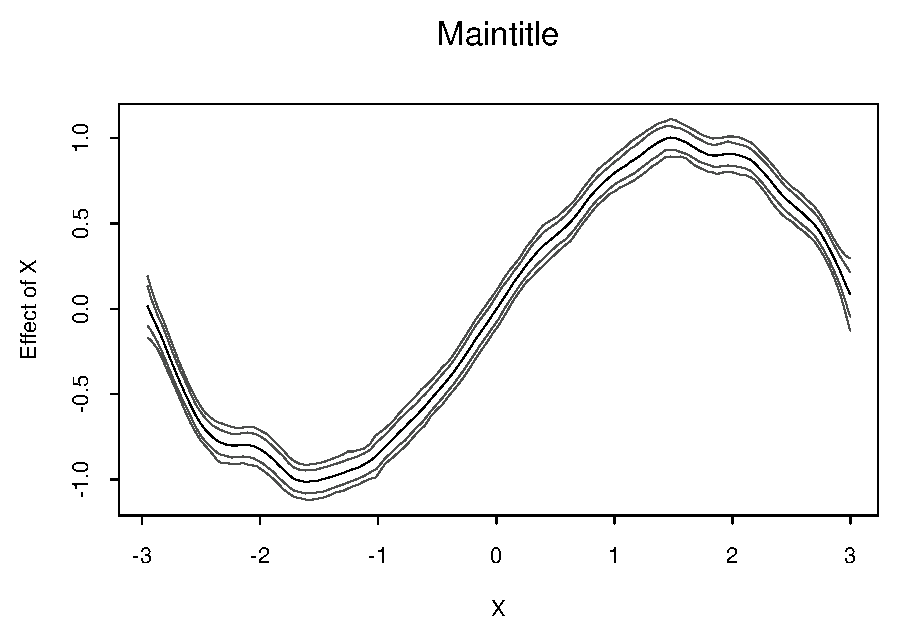
\includegraphics[scale=0.8]{grafiken/plotnonp.eps}
{\em\caption{ \label{illgraph} Illustration for the usage of
\em\tt plotnonp}}
\end{center}
\end{figure}

This statement draws the estimated effect of #X# and stores the
graph in the postscript file
#"c:#$\backslash$$\backslash$#bayes#$\backslash$$\backslash$#b_f_X_rw.ps"#.
A title, a x-axis and y-axis label is added to the graph. For
illustration purposes, the resulting graph is shown in
\autoref{illgraph}.

In some situations the effect of a covariate representing dates
must be plotted. Suppose for example that a covariate has values
ranging from 1 to 19 representing the time period from January
1983 to July 1984. In this case, we naturally prefer that the
x-axis is labelled in terms of dates rather than in the original
coding (from 1 to 19). To achieve this, function #plotnonp#
provides the three additional options #year#, #month# and #step#.
Options #year# and #month# are used to specify the year and the
month (1 for January, 2 for February, \dots) corresponding to the
minimum covariate value. In the example mentioned above
#year=1983# and #month=1# will produce the correct result. In
addition, option #step# may be specified to define the periodicity
in which your data are collected. For example #step=12# (the
default) corresponds to monthly data, while #step=4#, #step=2# and
#step=1# correspond to quarterly, half yearly and yearly data. We
illustrate the usage of #year#, #month# and #step# with our
example. Suppose we estimated the effect of calendar time #D#,
say, on a certain dependent variable, where the range of the data
is as described above. Then the following S-plus function call
will produce the postscript file shown in \autoref{illgraph2}:

\begin{figure}[ht]
\begin{center}
%\includegraphics[scale=0.8]{fvdate.eps}
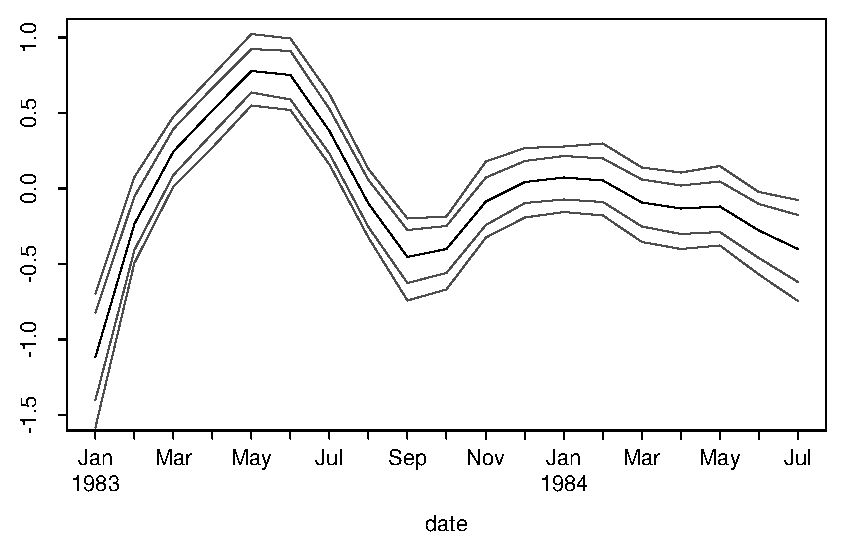
\includegraphics[scale=0.8]{grafiken/plotnonpdate.eps}
{\em\caption{ \label{illgraph2} Illustration for the usage of
\em\tt plotnonp}}
\end{center}
\end{figure}

#> plotnonp("c:\\bayes\\b_f_D_pspline.res", psname="c:\\bayes\\b_f_D_pspline.ps",#\\
#  year=1983,month=1,step=12,xlab="date", ylab= " ") #

Note, that \texttt{ylab=" "} forces S-plus to omit the y axis
label. If #ylab# (as well as #xlab#) is omitted, default labels
will be given to the two axis.

Finally, we note that all options that can be passed to the #plot#
function of S-plus may also be passed to function #plotnonp#.
Thus, function #plotnonp# is more or less a specialized version of
the S-plus #plot# function.


\subsubsection{Drawing geographical maps}
\index{S-plus!drawing geographical maps} \index{drawing
geographical maps}

This subsection describes how to visualize estimation results of
spatial covariates, where the observations represent the location
or site in connected geographical regions. A typical example for a
spatial covariate is given in the 'rents for flats' example, see
\autoref{rentdata}, where the covariate #L# indicates the location
(in subquarters) of the flat in Munich. \autoref{munich} shows a
map of Munich separated into subquarters.

\begin{figure}
\centering
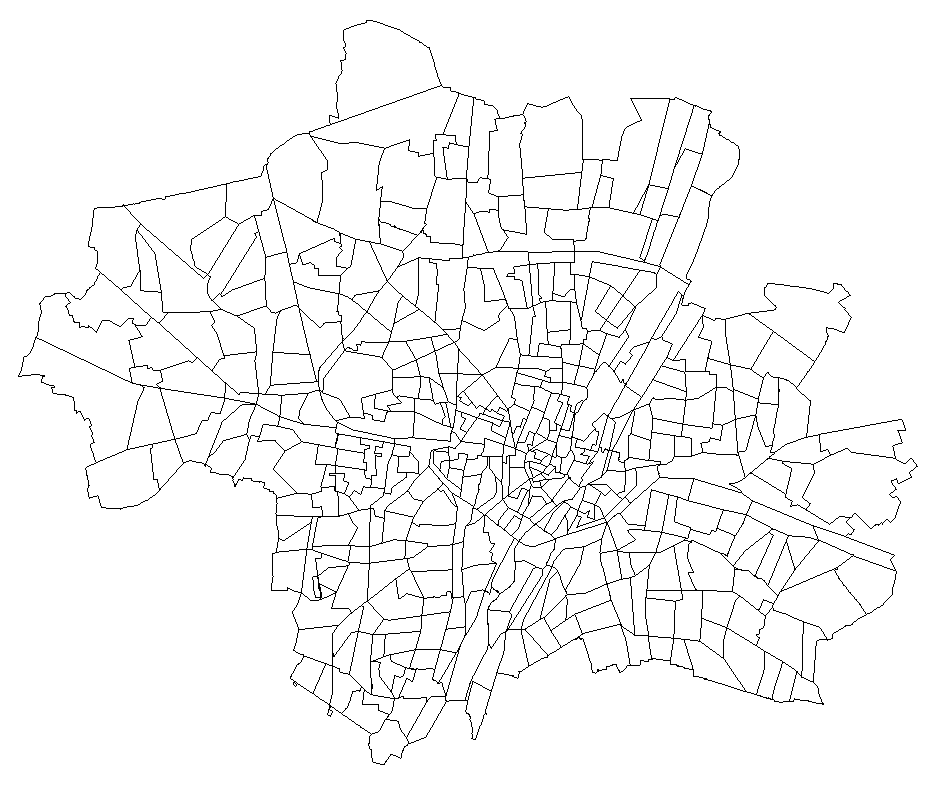
\includegraphics [scale=0.5]{grafiken/munich.eps}
{\em\caption{\label{munich} Map of Munich}}
\end{figure}


Typically, the effect of such a spatial covariate is incorporated
into a regression model via an unstructured or structured random
effect. In the latter case a spatial smoothness prior for the
spatial covariate is specified that penalizes too abrupt changes
of the estimated effect in neighboring sites. In some situations
the incorporation of both, an unstructured and a structured
effect, may also be appropriate. Details on how to incorporate
spatial covariates into a semiparametric regression  model are
given in \autoref{bayesregress}. For the rest of this section we
assume that an effect of a spatial covariate has already been
estimated and that we now want to visualize the estimation
results. This can be easily done with the two S-plus functions
#readbndfile# and #drawmap#. Function #readbndfile# is used to
read the boundary information of a map that is stored in a so
called boundary file and to store this information as a permanent
S-plus {\em map object}. The boundary file contains mainly the
polygons which form the different geographical regions of the map.
The required structure of such a file is described below. After
the successful reading of the boundary information of a map, the
second function #drawmap# may be used to draw and print the map
either on the screen or into a postscript file. There are several
possible ways to draw the map. In the simplest case the map can be
drawn without any estimation effects, i.e.~only the boundaries of
the different regions or sites are drawn, see \autoref{munich} for
an example. In practice, however, one usually wants to color the
regions of the map according to some numerical characteristics. As
an example compare \autoref{munichrelfreq} in which the
subquarters of Munich are colored according to the frequency of
flats in the 'rents for flats' data set located in the respective subquarter.
Subquarters colored in red contain less flats compared to
subquarters colored in green. In striped areas no observations are
available.

\begin{figure}[ht]
\begin{center}
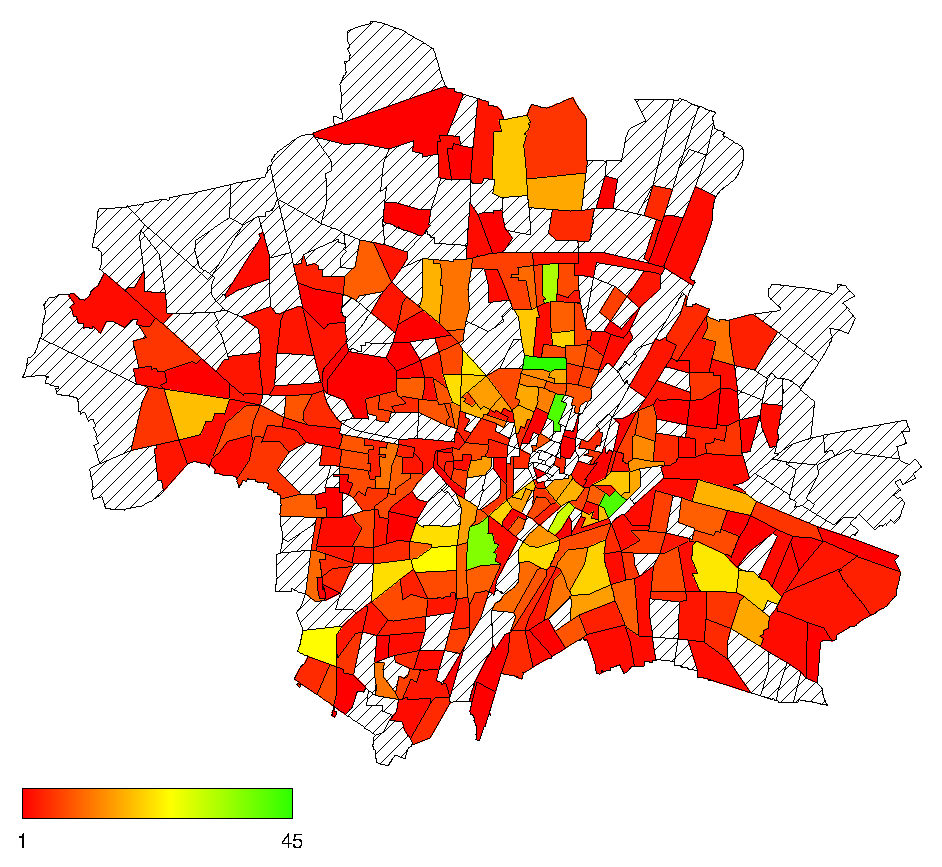
\includegraphics[scale=0.5]{grafiken/munichfr.eps}
{\em\caption{ \label{munichrelfreq} relative frequencies of
observed flats in the 'rents for flats' data set}}
\end{center}
\end{figure}


In the following we give a detailed description of the usage of
the functions #readbndfile# and #drawmap#.

{\bf Function readbndfile}
\medskip
\index{S-plus!reading boundary files} \index{reading boundary
files}

Function #readbndfile# is used to read in boundary information
stored in a boundary file into S-plus. The function has two
required arguments. The first argument is the filename of the
boundary file to read in. The second argument specifies the name
of the {\em map object} in S-plus (recall that the map information
is stored as a permanent S-plus object). To give an example,
suppose that {\em BayesX} is installed in the directory
#c:#$\backslash$#bayes# and that we want to read in the map of
Munich. In this case the boundary file of the map is stored in the
subdirectory #examples# of the installation directory, that is in
#c:#$\backslash$#bayes#$\backslash$#examples#. The name of the
boundary file is simply #munich.bnd#. The following function call
reads in the boundary information of Munich and stores the map
permanently in S-plus:

#> readbndfile("c:\\bayes\\examples\\munich.bnd","munich")#

Once again, note that double backslashes are required in S-plus to
specify a directory. The second argument in the statement above is
"munich", i.e.~the name of the map object is simply #munich#. To
refer to the map of Munich in subsequent statements and function
calls, the quotation marks must be omitted.

{\bf Function drawmap}
\medskip
\index{S-plus!drawmap}

Function #drawmap# is used to draw geographical maps and color the
regions according to some numerical characteristics. There is only
one required argument that must be passed to #drawmap#, that is
the name of the map to be drawn. Provided that the map has already
been read into S-plus (via function #readbndfile#), the following
statement draws the map of Munich in a S-plus graphic-window on
the screen:

#> drawmap(map=munich)#

Storing the map in a postscript file rather than drawing it on the
screen can be achieved by specifying the name of the postscript
file using the #outfile# option. For example the command

#> drawmap(map=munich,outfile="c:\\bayes\\munich.ps")#

produces a postscript file named #munich.ps# with the map of
Munich.

However, in most cases one not only wants to draw the boundaries
of a geographical map, but also color the regions according to
some numerical characteristics. Suppose for example that we have
already estimated a location specific effect on the monthly rents
in the 'rents for flats' data set. Suppose further that the
estimated effects are stored in
#c:#$\backslash$#bayes#$\backslash$#output#$\backslash$#b_f_L_spatial.res#.
The structure of the file is described in detail in
\autoref{bayesregress}. It contains 10 columns, one column with a
row counter, one column containing the values of the covariate
(here the location) and four columns containing estimated effects
for the values of the covariate. These are the posterior mean and
the posterior 2.5\%, 10\%, 50\%, 90\% and 97.5\% quantiles. The
last two columns contain posterior probabilities based on nominal
levels of 95\% and 80\%. The number 1 corresponds to a strictly
positive credible interval, the number -1 corresponds to a
strictly negative credible interval. A value of 0 indicates that
the corresponding credible interval contains zero. The first row
contains the column names. For the covariate #L# (location) for
example, the  first row of the file is given by:

 intnr   L  pmean   pqu2p5   pqu10   pmed   pqu90   pqu97p5 pcat95 pcat80

Suppose now that we want to visualize estimation results for the
spatial covariate #L# by coloring the subquarters of Munich
according to the estimated posterior mean. Compared to the S-plus
statement above, (at least) three more arguments must be passed to
function #drawmap#; the argument #dfile# that specifies the
filename of estimated results, the argument #plotvar# that
specifies the variable to be plotted and the argument #regionvar#
that specifies which column of the file, containing estimation
results, stores the region names. The following statement produces
the desired result:

 #> drawmap(map=munich,outfile="c:\\bayes\\munich.ps", #\\
 #  dfile="c:\\bayes\\output\\b_f_L_spatial.res", plotvar="pmean",regionvar="L")#


Note that the right hand side of options #plotvar# and #regionvar#
must be enclosed by quotation marks.

{\bf Optional arguments of function drawmap}

Besides the arguments discussed so far there are some more
optional arguments that can be passed to #drawmap#. They are
listed and described below together with a summary of the
arguments already described:


\begin{itemize}
\item {\bf map = characterstring}

Name of the S-plus {\em map object}. Use function #readbndfile# to
read in geographical maps into S-plus.
\item {\bf dfile = "filename (including path)"}

Filename (including path) of the file containing numerical
characteristics of the regions of the map. The file must contain
at least two columns, one column that lists the names of the
regions and one column containing the numerical characteristics of
the respective regions. It is important that the names of the
regions listed match with the region names stored in the S-plus
{\em map object}. The first row of the file must contain the names
of the columns.
\item {\bf outfile = "filename (including path)"}

Filename (including path) of the postscript file where the map
should be stored.
\item {\bf regionvar = "characterstring"}

Name of the column in the data file containing the region names
(see also argument #dfile#). Note that the right hand side must be
enclosed by quotation marks.
\item {\bf plotvar = "characterstring"}

Name of the column in the data file containing the numerical
characteristics of the regions (see also argument #dfile#). Note
that the right hand side must be enclosed by quotation marks.
\item {\bf lowerlimit = realvalue}

Lower limit of the range to be drawn. If #lowerlimit# is omitted,
the minimum numerical value in the #plotvar# column will be used
instead as the lower limit.
\item {\bf upperlimit = realvalue}

Upper limit of the range to be drawn. If #upperlimit# is omitted,
the maximum numerical value in the #plotvar# column will be used
instead as the upper limit.
\item {\bf nrcolors = integer}

To color the regions according to their numerical characteristics,
the data are divided into a (typically large) number of ordered
categories. Afterwards a color is associated with each category.
The #nrcolors# option can be used to specify the number of
categories (and with it the number of different colors). Default
value is 100.
\item {\bf pstitle = "characterstring"}

Adds a title to the graph. Note that the right hand side must be
enclosed by quotation marks.
\item {\bf color = T/F}

The #color# option allows to choose between a grey scale for the
colors and a colored scale. The default is #color=F#, which means
a grey scale.
\item {\bf legend = T/F}

By default a legend is drawn into the graph. To omit the legend in
the graph, #legend=F# must be passed as an additional argument.
\item {\bf drawnames = T/F}

In some situations it may be favorable to print the names of the
regions into the graph (although the result may be confusing in
most cases). This can be done by specifying the additional option
#drawnames=T#. By default the names of the regions are omitted in
the graph.
\item {\bf swapcolors = T/F}

In some situations it may be favorable to swap the order of the
colors, i.e.~red shades corresponding to large values and green
shades corresponding to small values. This is achieved by
specifying #swapcolors=T#. By default small values are colored in
red shades and large values in green shades.
\item {\bf pcat = T/F}

If you want to visualize the values of the columns #pcat80# or
#pcat95# it is convenient to specify #pcat=T#. This forces
#drawmap# to expect a column that consists only of the values -1,
0 and 1. Of course you can achieve the same result by setting
#nrcolors=3#, #lowerlimit=-1# and #upperlimit=1#. The default is
#pcat=F#.
\end{itemize}


\subsubsection{Plotting autocorrelation functions}
\label{splusplotautocor} \index{S-plus!plotting autocorrelation
functions} \index{plotting autocorrelation functions}
\index{autocorrelation functions!plotting}

This section describes how to visualize autocorrelation functions
of sampled parameters using the S-plus function #plotautocor#.

To compute autocorrelation functions, the post-estimation command
#autocor# must be applied, see \autoref{bayesautocorr} for
details. For the rest of this section we assume that
autocorrelations are already computed and stored in file:

#c:#$\backslash$#bayes#$\backslash$#output#$\backslash$#b_autocor.raw#

The minimum number of arguments required for the function is one,
namely the file where the computed autocorrelation functions are
stored. In this case a S-plus {\em graphic window} will be opened
and the autocorrelation functions are plotted on the screen. To
store autocorrelations in a postscript file, an output filename
must be specified as a second argument. Thus, the S-plus command

#> plotautocor("c:\\bayes\\output\\b_autocor.raw")#

prints autocorrelations on the screen, while the statement

 #> plotautocor("c:\\bayes\\output\\b_autocor.raw","c:\\bayes\\output\\b_autocor.ps")#

forces S-plus to store the autocorrelation graphs in the
postscript file #c:\bayes\output\b_autocor.ps#.

In particular for regression models with a large number of
parameters the execution of function #plotautocor# can be very
time consuming. Moreover, the size of the resulting postscript
file can be very large. To avoid such problems #plotautocor#
provides the additional argument #mean.autocor#. If
#mean.autocor=T# is specified, for each lag number and model term
only minimum, mean and maximum autocorrelations are plotted,
leading in most cases to a considerable reduction in computing
time and storing size.


\subsubsection{Plotting sampled parameters}
\label{splusplotsample} \index{S-plus!plotting sampled parameters}
\index{plotting sampled parameters}

This section describes how to plot sampled parameters using the
S-plus function #plotsample#. Before applying function
#plotsample#, sampled parameters must be stored in ASCII-format
using the post-estimation command #getsample#. See
\autoref{bayesgetsample} for details, but note that sampled
parameters will be stored in several different files, typically
one file for each term in the model.

Suppose now that we want to visualize sampling paths for the
parameters of the nonlinear effect of a covariate X. Assume
further that sampled parameters are stored in the ASCII file

#c:\bayes\output\b_X_sample.raw#.

As most other functions, #plotsample# provides two possibilities
of drawing sampled parameters. The first possibility is to print
the graphs on the screen, and the second is to store them into a
postscript file. To print the sampling paths on the screen, only
the filename (including path) of the ASCII file where sampled
parameters are stored must be passed to the function. For the
example mentioned above the corresponding command is:

#> plotsample("c:\\bayes\\output\\b_X_sample.raw")#

If sampling paths should be drawn into a postscript file rather
than on the screen, the filename of the resulting postscript file
must be specified as a second argument. Thus, for our example we
get:

 #> plotsample("c:\\bayes\\output\\b_X_sample.raw","c:\\bayes\\output\\b_X_sample.ps")#

In addition, all options that are available for the S-plus
function #plot# may be passed to function #plotsample#, see the
S-plus documentation for details.


\subsubsection{Plotting 2 dimensional surfaces}

This subsection describes the usage of the function #plotsurf# for
visualizing 2 dimensional surfaces. The function #plotsurf# merely
invokes different S-plus functions for visualizing 2 dimensional
data. Thus, users familiar with S-plus may prefer to use this
functions directly to gain more flexibility. Note that this function
is only available for S-plus.

Suppose that a Bayesian regression model has already been
estimated with predictor

$$
\eta = \dots + f(X1,X2) + \dots,
$$

where the interaction effect of #X1# and #X2# is modelled
nonparametrically using 2 dimensional P-splines and that the
estimation results are stored in file:

#c:\bayes\output\b_f_X1_X2_pspline.res#

The S-plus function #plotsurf# requires at least one argument,
which is the name (including path) of the file containing the
estimation results. For example the command

#> plotsurf("c:\\bayes\\output\\b_f_X1_X2_pspline.res")#

prints the posterior means against #X1# and #X2# on the screen.
There are several additional options that can be passed, for
example for changing the plot type or storing the graph as a
postscript file rather than displaying it on the screen. The
following list describes all possible arguments that may be passed
to the function #plotsurf#:

\begin{itemize}
\item {\bf data = "filename (including path)"}

Name (including path) of the file containing the estimation
results. The file must contain at least 3 columns, one for the
x-axis, one for the y-axis and one for the z-axis. The file must
contain a header.
\item {\bf outfile = "filename (including path)"}

Name (including path) of the postscript file where the graph
should be stored. This option is only meaningful for #mode=2# and
#mode=3#.
\item {\bf cols = 3 column vector}

This option is only meaningful, if the argument #data# is
specified. In this case #cols# gives the columns of the object or
data file passed to the argument #data#, that should be used as
values for the x, y and z axis. The default is #cols=c(2,3,4)#
which corresponds to plotting the posterior means against #X1# and
#X2#.
%\item {\bf zlim = 2 column vector}

%2 column vector giving the minimum and maximum value to be put on
%the z-axis.
\item {\bf mode = 1/2/3/4/5}

This option specifies the plot type. Currently there are 5
different types available. The default is #mode=1#, which
corresponds to what is called a 'Surface Plot' in S-plus.
\end{itemize}


\section{Global options}
\label{bayesregglobopt} \index{bayesreg object!global options}

The purpose of global options is to affect the global behavior of
a {\em bayesreg object}. The main characteristic of global options
is, that they are not associated with a certain method.

The syntax for specifying global options is

#> #{\em objectname}.{\em optionname} = {\em newvalue}

where {\em newvalue} is the new value of the option. The type of
the value depends on the respective option.

The following global options are currently available for {\em
bayesreg objects}:

\begin{itemize}
\item {\bf outfile = filename} \\
By default, the estimation output produced by the #regress#
procedure will be written to the default output directory, which
is

$<$#INSTALLDIRECTORY#$>$$\backslash$#output#.

The default filename is composed of the name of the {\em bayesreg
object} and the type of the file. For example, if you estimated a
nonparametric effect for a covariate #X#, say, then the estimation
output will be written to

$<$#INSTALLDIRECTORY#$>$$\backslash$#output#$\backslash$#b_nonpX.res#

where #b# is the name of the {\em bayesreg object}. In most cases,
however, it may be necessary to save estimation results into a
different directory and/or under a different filename than the
default. This can be done using the #outfile# option. With the
#outfile# option you have to specify the directory where the
output should be stored to and in addition a base filename. The
base filename should not be a complete filename. For example
specifying

#> b.outfile = c:\data\res#

would force {\em BayesX} to store the estimation result for the
nonparametric effect of #X# in file

#c:\data\res_nonpX.res#

\item {\bf iterationsprint = integer}

By default, the current iteration number is printed in the {\em
output window} (or in an additional log file) after every 100th
iteration. This can lead to rather big and complex output files.
The #iterationsprint# option allows to redefine after how many
iterations the current iteration number is printed. For example
#iterationsprint=1000# forces {\em BayesX} to print the current
iterations number only after every 1000th iteration rather than
after every 100th iteration.
\end{itemize}



\section{Examples}
\label{bayesregexamples}

In this Section we present a couple of complex examples about the
usage of {\em bayesreg objects}. The first example contains a
reanalysis of the 'credit scoring' data set that is described in
\autoref{creditdata}, which contains also a (incomplete) list of
some publications where the 'credit scoring' data set has already
been analyzed. The second example is a Bayesian analysis of
determinants of childhood undernutrition in Zambia. The data set
is described in \autoref{zambia}. This section contains also a
list of publications where the data set has been analyzed. Both
data sets are shipped together with {\em BayesX} and are stored in
the directory #examples#, which is a subdirectory of the
installation directory. Since the main focus here is on
illustrating the usage of {\em bayesreg objects}, we omit any
interpretation of estimated effects.


\subsection{Binary data: credit scoring}
\label{creditanalyse}

All {\em BayesX} statements of this section can be found in the
#examples# directory in the file #credit.prg#. In principle, the
commands in #credit.prg# can be executed using the #usefile#
command for running batch files, see \autoref{batch}. Note,
however, that the specified directories therein may not exist on
your computer. Thus, to avoid errors, the file must be modified
first to execute correctly.

\subsubsection{Reading the data into BayesX}


In order to analyze the 'credit scoring' data set, we first have
to load the data set into {\em BayesX}. For the rest of this
section we assume that {\em BayesX} is installed in the directory
#c:#$\backslash$#bayes#. In this case, the 'credit scoring' data
set can be found in #c:#$\backslash$#bayes#$\backslash$#examples#
under the name #credit.raw#. With the following two commands
(entered in the {\em command window}) we first create a {\em
dataset object} #credit# and afterwards load the data set into
{\em BayesX} using the #infile# command:

#> dataset credit# \\
#> credit.infile using c:\bayes\examples\credit.res#

Since the first row of the file already contains the variable
names, it is not necessary to specify variable names in the
#infile# statement. If the first row of the data set does not
contain the variable names, they must be additionally specified in
the #infile# command, e.g.~for the 'credit scoring' data set we
get

#> credit.infile y account duration amount payment intuse marstat# \\
#  using c:\bayes\examples\credit.res#


We now compute effect coded versions of the categorical covariates
#account#, #payment#, #intuse# and #marstat#:

#> credit.generate account1  = 1*(account=1)-1*(account=3)# \\
#> credit.generate account2  = 1*(account=2)-1*(account=3)# \\
#> credit.generate payment1 = 1*(payment=1)-1*(payment=2)# \\
#> credit.generate intuse1 = 1*(intuse=1)-1*(intuse=2)# \\
#> credit.generate marstat1 = 1*(marstat=1)-1*(marstat=2)#

The reference categories for the covariates are chosen to be 3 for
#account# and 2 for the others.

\subsubsection{Creating a bayesreg object}

Before we are able to estimate Bayesian regression models, we
first have to create a {\em bayesreg object}:

#> bayesreg b# \\
#> b.outfile = c:\results\credit#

The second command changes the default output directory and name
(which is #c:\bayes\output\b#) to
#c:\results\credit#. This means that
subsequent regression output is stored in the directory
#c:\results# and that all filenames start with
#credit#.

\subsubsection{Probit models}

\label{credit_probit} We can now start estimating models. We first
describe how probit models are estimated. The estimation of probit
models is slightly faster than logit models because the full
conditionals of the effects are Gaussian.

We first estimate a model with fixed effects only:

#> b.regress  y = account1 + account2 + duration + amount + payment1 + intuse1 #\\
#  + marstat1, predict iterations=6000 burnin=1000 step=5 family=binomialprobit # \\
#  using credit #

Here we specified 6000 iterations, a burnin period of 1000
iterations and a thinning parameter of 5, i.e.~every 5th sampled
parameter will be stored and used for estimation. The additional
option \hyperref[predict]{#predict#} is used to compute samples of
the deviance, the effective number of parameters, the deviance
information criteria (DIC), predicted means etc.

Executing the command yields the following output (simulation
output omitted):

\small

\begin{verbatim}

SIMULATION TERMINATED

SIMULATION RUN TIME: 13 seconds


ESTIMATION RESULTS:

  Predicted values:

  Estimated mean of predictors, expectation of response and
  individual deviances are stored in file
  c:\results\credit_predictmean.raw

  Estimation results for the Deviance:

  Unstandardized Deviance (-2*Loglikelihood(y|mu))

  Mean:             1027.05
  Std. Dev:         4.22501
  2.5% Quantile:    1021.01
  10% Quantile:     1022.48
  50% Quantile:     1026.29
  90% Quantile:     1032.73
  97.5% Quantile:   1037.28

  Saturated Deviance (-2*Loglikelihood(y|mu) + 2*Loglikelihood(y|mu=y))

  Mean:             1027.05
  Std. Dev:         4.22501
  2.5% Quantile:    1021.01
  10% Quantile:     1022.48
  50% Quantile:     1026.29
  90% Quantile:     1032.73
  97.5% Quantile:   1037.28

  Samples of the deviance are stored in file
  c:\results\credit_deviance_sample.raw

  Estimation results for the DIC:

  DIC based on the unstandardized Deviance

  Deviance(bar_mu):           1018.85
  pD:                         8.20049
  DIC:                        1035.26

  DIC based on the saturated Deviance

  Deviance(bar_mu):           1018.85
  pD:                         8.20049
  DIC:                        1035.26




  FixedEffects1


  Acceptance rate:    100 %


  Variable  mean           Std. Dev.      2.5% quant.    median         97.5% quant.
  const     -0.715437      0.117673       -0.9464        -0.710836      -0.49298
  account1  -0.629553      0.0684571      -0.764526      -0.6244        -0.50343
  account2  0.50699        0.0625032      0.389608       0.506698       0.63888
  duration  0.0204795      0.00471734     0.0111948      0.0205776      0.0298505
  amount    0.0172111      0.0189096      -0.0173778     0.0167277      0.0542619
  payment1  -0.2919        0.0762402      -0.438703      -0.288309      -0.152512
  intuse1   -0.137287      0.0477423      -0.228492      -0.137755      -0.041511
  marstat1  -0.158195      0.0476991      -0.254198      -0.157534      -0.0663364

  Results for fixed effects are also stored in file
  c:\results\credit_FixedEffects1.res
\end{verbatim}


\normalsize

Somewhat surprisingly, we observe that the amount of credit seems
to have no ('significant') influence on the response. To check
this phenomenon more carefully, we run a second estimation, now
allowing for possibly nonlinear effects of the continuous
covariates #amount# and #duration#. We choose cubic P-splines with
second order random walk penalty as smoothness priors and modify
the #regress# statement above according to the new model:

#> b.regress  y = account1 + account2 + duration(psplinerw2) + amount(psplinerw2)# \\
#  + payment1 + intuse1 + marstat1, predict iterations=6000 burnin=1000 step=5# \\
#  family=binomialprobit using credit #

We get the following output for the nonlinear functions (output
for the rest omitted):

\small

\begin{verbatim}

  f_duration_pspline


  Acceptance rate:    100 %

  Results are stored in file c:\results\credit_f_duration_pspline.res

  Postscript file is stored in file c:\results\credit_f_duration_pspline.ps

  Results may be visualized using method 'plotnonp'
  Type for example: objectname.plotnonp 1


  f_duration_pspline_variance


  Acceptance rate:    100 %

  Estimation results for the variance component:

  Mean:             0.00787338
  Std. dev.:        0.0100301
  2.5% Quantile:    0.00128376
  10% Quantile:     0.00190016
  50% Quantile:     0.00487717
  90% Quantile:     0.0157856
  97.5% Quantile:   0.0315107

  Results for the variance component are also stored in file
  c:\results\credit_f_duration_pspline_var.res


  f_amount_pspline


  Acceptance rate:    100 %

  Results are stored in file c:\results\credit_f_amount_pspline.res

  Postscript file is stored in file c:\results\credit_f_amount_pspline.ps

  Results may be visualized using method 'plotnonp'
  Type for example: objectname.plotnonp 3


  f_amount_pspline_variance


  Acceptance rate:    100 %

  Estimation results for the variance component:

  Mean:             0.00870842
  Std. dev.:        0.0115895
  2.5% Quantile:    0.0013844
  10% Quantile:     0.00220351
  50% Quantile:     0.00570725
  90% Quantile:     0.0164858
  97.5% Quantile:   0.0340326

  Results for the variance component are also stored in file
  c:\results\credit_f_amount_pspline_var.res
\end{verbatim}


\normalsize


We  visualize estimated effects for #amount# and #duration# using
method #plotnonp# (as advised by the program):

#> b.plotnonp 1 , outfile="c:\results\credit_duration.ps"#\\
#> b.plotnonp 3 , outfile="c:\results\credit_amount.ps"#

This produces the graphs (stored in postscript files) shown in
\autoref{creditfigures}.

\begin{figure}[ht]
\vspace{0.5cm}
\begin{center}
\includegraphics[scale=0.65]{grafiken/credit_duration.ps}

\vspace{0.5cm}
\includegraphics[scale=0.65]{grafiken/credit_amount.ps}
\end{center}
{\em\caption{ \label{creditfigures} Estimated effects of duration
and amount of credit. Shown is the posterior mean within 80\% and
95\% credible regions.}}
\end{figure}

We add a title, x-axis and y-axis labels by typing \hfill

#> b.plotnonp 1 , outfile="c:\results\credit_duration.ps" replace #\\
#  xlab="duration" ylab="f(duration)" title="effect of duration"#

#> b.plotnonp 3 , outfile="c:\results\credit_amount.ps" replace# \\
#  xlab="amount" ylab="f(amount)" title="effect of amount"#

and obtain the improved graphs shown in \autoref{creditfigures_2}.
The option #replace# is specified to allow {\em BayesX} to
overwrite the previously generated postscript files. If the
#outfile# option is omitted, the graphs are printed on the screen
rather than being stored as postscript files.

\begin{figure}[ht]
\vspace{0.5cm}
\begin{center}
\includegraphics[scale=0.65]{grafiken/credit_duration_2.ps}

\vspace{0.5cm}
\includegraphics[scale=0.65]{grafiken/credit_amount_2.ps}
\end{center}
{\em\caption{ \label{creditfigures_2} Improved plots of the effect
of {\em\tt duration} and {\em\tt amount}.}}
\end{figure}


We now want to check the mixing of the generated Markov chains,
although the mixing for probit models is usually excellent. For
that reason we compute and plot the autocorrelation functions by
typing:

#> b.plotautocor , outfile="c:\results\credit_autocor.ps"#

We obtain the file
#c:#$\backslash$#results#$\backslash$#credit_autocor.ps# containing 9
pages of autocorrelation functions for all parameters in the
model. The first page of this file is shown in
\autoref{credit_autocor1}. We see that autocorrelations die off
very quickly.

\begin{figure}[ht]
\vspace{0.5cm}
\begin{center}
\includegraphics[scale=0.8]{grafiken/credit_autocor1.ps}
\end{center}
{\em\caption{ \label{credit_autocor1} First page of the
autocorrelation file.}}
\end{figure}

\clearpage

\subsubsection{Logit models}

A logit model rather than a probit model is estimated by replacing
#family=binomialprobit# with #family=binomial#:

#> b.regress  y = account1 + account2 + duration(psplinerw2) + amount(psplinerw2)# \\
#  + payment1 + intuse1 + marstat1, predict iterations=6000 burnin=1000 step=5# \\
#  family=binomial using credit#

In contrast to binary probit models, the full conditionals for the
regression coefficients are no longer Gaussian. {\em BayesX}
offers 3 different types of proposal densities. These are
iteratively weighted least squares (IWLS) proposals based either
on the current state of the parameters or on the posterior modes
as described in \autoref{IWLS} or Brezger and Lang (2003), and
conditional prior proposals as described in Fahrmeir and Lang
(2001b). We recommend the usage of IWLS proposals, since no tuning
is required and mixing properties are superior to those of
conditional prior proposals. The default are IWLS proposals based
on the current state of the parameters. The following statement
causes {\em BayesX} to use IWLS proposals based on posterior
modes, which usually yield even higher acceptance probabilities
compared to ordinary IWLS proposals:

#> b.regress  y = account1 + account2 + duration(psplinerw2,proposal=iwlsmode)# \\
#  + amount(psplinerw2,proposal=iwlsmode) + payment1 + intuse1 + marstat1,# \\
#  predict iterations=6000 burnin=1000 step=5# \\
#  family=binomial using credit#

As for the probit model, we visualize the estimated nonlinear
effects of #duration# and #amount# using method #plotnonp#:

#> b.plotnonp 1 , outfile="c:\results\credit_logit_duration.ps" replace# \\
#  xlab="duration" ylab="f(duration)" title="effect of duration" #

#> b.plotnonp 3 , outfile="c:\results\credit_logit_amount.ps" replace# \\
#  xlab="amount" ylab="f(amount)" title="effect of amount" #

The resulting graphs are shown in \autoref{creditlogit}. As could
have been expected only the scale of the estimated effects differs
(because of the logit link).

\begin{figure}[ht]
\vspace{0.5cm}
\begin{center}
\includegraphics[scale=0.65]{grafiken/credit_logit_duration.ps}

\vspace{0.5cm}
\includegraphics[scale=0.65]{grafiken/credit_logit_amount.ps}
\end{center}
{\em\caption{ \label{creditlogit} Effect of {\em\tt duration} and
{\em\tt amount}, if a logit model is estimated rather than a
probit model.}}
\end{figure}

Once again, to check the mixing of the sampled parameters we
compute and plot the autocorrelation functions using method
#plotautocor#:

#> b.plotautocor , outfile="c:\results\credit_logit_autocor.ps"#

The first page of the resulting postscript file is shown in
\autoref{creditautocorlogit_1}. As can be seen, the
autocorrelations for the logit model with IWLS proposals are
almost as low as for the probit model.

\begin{figure}[ht]
\vspace{0.5cm}
\begin{center}
\includegraphics[scale=0.8]{grafiken/credit_logit_autocor1.ps}
\end{center}
{\em\caption{ \label{creditautocorlogit_1} First page of the
autocorrelation file, if a logit model is estimated.}}
\end{figure}

\clearpage

\subsubsection{Varying the hyperparameters}

In the preceding examples we used the default hyperparameters
#a=0.001# and #b=0.001# for the inverse gamma prior of the
variances. In some situations, however, the estimated nonlinear
functions may considerably depend on the particular choice of
hyperparameters #a# and #b#. This may be the case for very low
signal to noise ratios or/and small sample sizes. It is therefore
highly recommended to estimate all models under consideration
using a (small) number of {\em different} choices for #a# and #b#
(e.g.~#a=1#,#b=0.005#; #a=0.001#,#b=0.001#; #a=0.0001#,#b=0.0001#)
to assess the dependence of results on minor changes in the model
assumptions. In that sense, the variation of hyperparameters can
be used as a tool for model diagnostics.

We estimate our probit model from \autoref{credit_probit} again,
but now with hyperparameters #a=1.0#, #b=0.005# and #a=0.0001#,
#b=0.0001#, respectively.

 #> b.regress  y = account1 + account2 + duration(psplinerw2,a=1.0,b=0.005) +# \\
 #  amount(psplinerw2,a=1.0,b=0.005) + payment1 + intuse1 + marstat1,# \\
 #  predict iterations=6000 burnin=1000 step=5 family=binomialprobit using credit #

 #> b.regress  y = account1 + account2 + duration(psplinerw2,a=0.0001,b=0.0001) +# \\
 #  amount(psplinerw2,a=0.0001,b=0.0001) + payment1 + intuse1 + marstat1, #\\
 #  predict iterations=6000 burnin=1000 step=5 family=binomialprobit using credit#

\autoref{credit_varhyper} shows the estimated nonlinear effects of
variables #duration# and #amount# with the different choices for
#a# and #b#. We see that in this example estimation results differ
only slightly for the different choices of #a# and #b#.


\begin{figure}[ht]
\vspace{0.5cm}
\begin{center}
\includegraphics[scale=0.4]{grafiken/credit_duration_a001b001.ps} \hspace{0.3cm}
\includegraphics[scale=0.4]{grafiken/credit_amount_a001b001.ps}

\vspace{0.5cm}
\includegraphics[scale=0.4]{grafiken/credit_duration_a1b005.ps} \hspace{0.3cm}
\includegraphics[scale=0.4]{grafiken/credit_amount_a1b005.ps}

\vspace{0.5cm}
\includegraphics[scale=0.4]{grafiken/credit_duration_a0001b0001.ps} \hspace{0.3cm}
\includegraphics[scale=0.4]{grafiken/credit_amount_a0001b0001.ps}
\end{center}
{\em\caption{ \label{credit_varhyper} Results for the effect of
{\em\tt duration} and {\em\tt amount} for different values of the
hyperparameters for the variances.}}
\end{figure}


\clearpage

\subsection{Determinants of childhood undernutrition in Zambia}

\label{zambiaanalysis} In this subsection we present a tutorial
like example for the usage of {\em bayesreg objects}. We use data
on undernutrition of children in Zambia, compare \autoref{zambia}
for a description of the data set. The files containing the data
and the map can be found in the subdirectory #examples# of the
installation directory together with the batch file
#mcmctutorial.prg# containing all commands used in the following
subsections.

The rest of the example is separated in seven parts dealing with
the different steps of estimating a regression model. In
\autoref{zambia_mcmc_datasets} we create a {\em dataset object} to
incorporate, handle and manipulate the data. We will also give a
brief description of some methods that may be applied to {\em
dataset objects}. Since we want to estimate a spatial effect of
the district in which a child lives, we need the boundaries of the
districts to compute the neighborhood information of the map of
Zambia. This information will be stored in a {\em map object}.
\autoref{zambia_mcmc_maps} describes how to create and handle
these objects. Estimation of the regression model is carried out
in \autoref{zambia_mcmc_regression} using a {\em bayesreg object}.
The next two sections describe how to visualize the estimation
results and how to customize the obtained graphics.
\autoref{zambia_mcmc_postest} describes post estimation commands
which can be used to investigate the sampling paths and the
autocorrelation functions of the estimated parameters. In a last
section we perform a sensitivity analysis to assess the impact of
hyperparameter choices on our estimation results.

Please note, that all paths within the following subsections must
be changed according to the storage location of the corresponding
files on your hard disk.

\subsubsection{Reading data set
information}\label{zambia_mcmc_datasets}

In a first step we read the available data set information into
{\it BayesX}. Therefore we create a {\it dataset object} named
#d#:

#> dataset d#

We store the data in #d# using the method #infile#:

#> d.infile, maxobs=5000 using c:\data\zambia.raw#

Note, that we assume the data to be provided in the external file
#c:\data\zambia.raw#. The first few lines of this file look like
this:

{\footnotesize
 hazstd bmi agc district rcw edu1 edu2 tpr sex\\
 0.0791769 \,\, 21.83 \,\, 4 \,\, 81 \,\, -1 \,\, 1 \,\, 0 \,\, 1 \,\, -1\\
 -0.2541965 \,\, 21.83 \,\, 26 \,\, 81 \,\, -1 \,\, 1 \,\, 0 \,\, 1 \,\, -1\\
 -0.1599823 \,\, 20.43 \,\, 56 \,\, 81 \,\, 1 \,\, -1 \,\, -1 \,\, 1 \,\, 1\\
 0.1733911 \,\, 22.27 \,\, 6 \,\, 81 \,\, -1 \,\, 0 \,\, 1 \,\, 1 \,\, 1}

In our example the file contains the variable names in the first
line. Therefore it is not necessary to specify them in the
#infile# command. If the file contained only the data without
variable names, we would have to supply them after the keyword
#infile#:

 #> d.infile hazstd bmi agc district rcw edu1 edu2 tpr sex, maxobs=5000#
 #  using c:\data\zambia.raw#


Option #maxobs# can be used to speed up the execution time of the
#infile# command. If #maxobs# is specified, {\it BayesX} allocates
enough memory to store all the data while the total amount of
required memory is unknown in advance if #maxobs# remains
unspecified. For larger data sets this may cause {\it BayesX} to
start reading the data set information several times because the
currently allocated memory is exceeded. However, this is only
meaningful for larger data sets with more than 10000 observations
and could therefore be omitted in our example.

A second option that may be added to the #infile# command is the
#missing# option to indicate missing values. Specifying for
example {\tt missing=M} defines the letter '{\tt M}' as an
indicator for a missing value. The default for missing values are
a period '.' and '{\tt NA}' (which remain valid indicators for
missing values even if an additional indicator is defined by the
{\tt missing} option).

After having read in the data set information we can inspect the
data visually. Executing the command

#> d.describe#

opens an {\it object-viewer window} containing the data in form of
a spreadsheet. This can also be achieved by double-clicking on the
{\it dataset object} in the {\it object browser}.

Further methods allow to examine the variables in the {\it dataset
object}. For a categorial variable, e.g.~#sex#, the #tabulate#
command may be used to produce a frequency table:

#> d.tabulate sex#

resulting in

\begin{verbatim}
Variable: sex

          Value       Obs           Freq            Cum
             -1      2451         0.5057         0.5057
              1      2396         0.4943              1
\end{verbatim}

being printed in the {\it output window}. For continuous variables
the #descriptive# command prints several characteristics of the
variable in the {\em output window}. E.g., executing

#> d.descriptive bmi#

leads to

\begin{verbatim}
   Variable    Obs        Mean      Median         Std         Min         Max
        bmi   4847   21.944349        21.4   3.2879659        12.8       39.29
\end{verbatim}

\subsubsection{Map objects}\label{zambia_mcmc_maps}

In the following we want to estimate a spatially correlated effect
of the district in which a child lives. Therefore we need the
boundaries of the districts in Zambia to compute the neighborhood
information of the map of Zambia. We therefore create a {\it map
object}

#> map m#

and read in the boundaries using the #infile# command of {\it map
objects}:

#> m.infile using c:\data\zambia.bnd#

Having read in the boundary information, {\it BayesX}
automatically computes the neighborhood matrix of the map.

The file following the keyword #using# is assumed to contain the
boundaries in form of closed polygons. Compare \autoref{map} for a
description of the expected file format.

{\it Map objects} may be visualized using method #describe#:

#> m.describe#

resulting in the graph shown in \autoref{zambia_mcmc_zambiamap}.
Additionally, #describe# prints further information about the {\it
map object} in the {\it output window} including the name of the
object, the number of regions, the minimum and maximum number of
neighbors and the bandwidth of the corresponding adjacency or
neighborhood matrix:

\begin{verbatim}
  MAP m
  Number of regions: 54
  Minimum number of neighbors: 1
  Maximum number of neighbors: 9
  Bandsize of corresponding adjacency matrix: 24
\end{verbatim}

\begin{figure}[ht]
\begin{center}
\epsfig{file=grafiken/zambia.ps,scale=0.35} {\it\caption{The
districts within Zambia.\label{zambia_mcmc_zambiamap}}}
\end{center}
\end{figure}


The numerical complexity associated with the estimation of
structured spatial effects using MCMC techniques depends
essentially on the structure of the neighborhood matrix. Often the
geographical information stored in a boundary file does not
represent the 'ideal' ordering (as regards to the estimation
problem) of the districts or regions. Therefore it may be useful
to reorder the map using method #reorder#:

#> m.reorder#

Usually reordering results in a smaller bandwidth although the
bandwidth is not the criterion that is minimized by #reorder#.
Instead the {\it envelope} of the neighborhood matrix is minimized
(compare George and Liu 1981).

In order to avoid reordering the {\it map object} every time you
start {\it BayesX} it is useful to store the reordered version in
a separate file. This can be achieved using the #outfile# command
of {\it map objects}:

#> m.outfile, replace using c:\data\zambiasort.bnd#

The reordered map is now stored in the given file. Note, that
specifying the option #replace# allows {\it BayesX} to overwrite
an existing file with the same name. Without this option an error
message would be raised if the given file is already existing.

Reading the boundary information from an external file and
computing the neighborhood matrix may be a computationally
intensive task if the map contains a large number of regions or if
the polygons are given in great detail. To avoid doing these
computation in every $BayesX$ session, we store the neighborhood
information in a so-called {\it graph file} using method #outfile#
together with the #graph# option (compare \autoref{map} for a
description of {\em graph files}):

#> m.outfile, replace graph using c:\data\zambiasort.gra#

To see how storing maps in {\it graph files} affects the
computation time of the #infile# command, we create a second {\it
map object} and read in the information from the graph file.
Again, we have to specify the keyword #graph#:

#> map m1#\\
#> m1.infile, graph using c:\data\zambiasort.gra#

As you should have noticed, reading geographical information from
a {\it graph file} is usually much faster than reading from a {\it
boundary file}. However, using {\it graph files} also has a
drawback. Since they do no longer contain the full information on
the polygons forming the map, we can not visualize a {\it map
object} created from a {\it graph file}. Trying to do so

#> m1.describe#

raises an error message. This implies, that visualizing estimation
results of spatial effects can only be based on {\it map objects}
created from {\it boundary files}, although estimation can be
carried out using {\it graph files}. Since we will work with the
{\it map object} #m# in the following, we delete #m1#:

#> drop m1#

\subsubsection{Bayesian semiparametric
regression}\label{zambia_mcmc_regression}

To estimate a regression model using MCMC techniques we first
create a {\it bayesreg object}:

#> bayesreg b#

By default estimation results are written to the subdirectory
#output# of the installation directory. In this case the default
filenames are composed of the name of the {\it bayesreg object}
and the type of the specific file. Usually it is more convenient
to store the results in a user-specified directory. To define this
directory we use the #outfile# command of {\it bayesreg objects}:

#> b.outfile = c:\data\b#

Note, that #outfile# does not only specify a directory but also a
base filename (the character #b# in our example). Therefore
executing the command above leads to storage of the results in the
directory #c:\data# and all filenames start with the character
#b#. Of course the base filename may be different from the name of
the {\it bayesreg object}.

In addition to parameter estimates {\it BayesX} also gives
acceptance rates for the different effects and some further
information on the estimation process. In contrast to parameter
estimates this information is not stored automatically but is
printed in the {\it output window}. Therefore it is useful to
store the contents of the {\it output window}. This can be
achieved automatically by opening a log file using the #logopen#
command

#> logopen, replace using c:\data\logmcmc.txt#

After opening a log file, every information written to the {\em
output window} is also stored in the log file. Option #replace#
allows {\it BayesX} to overwrite an existing file with the same
name as the specified log file. Without #replace# results are
appended to an existing file.

The model presented in Kandala et al.~(2001) is given by the
following semiparametric predictor:
\[\eta=\gamma_0+\gamma_1rcw+\gamma_2edu1+\gamma_3edu2+\gamma_4tpr+\gamma_5sex+f_1(bmi)+f_2(agc)+f^{str}(district)+f^{unstr}(district)\]
The two continuous covariates #bmi# and #agc# are assumed to have
a possibly nonlinear effect on the Z-score and are therefore
modelled nonparametrically (as P-splines with second order random
walk prior in our example). The spatial effect of the district is
split up into a spatially correlated part $ f^{str}(district)$ and
an uncorrelated part $f^{unstr}(district)$, see Fahrmeir and Lang
(2001b) for a motivation. The correlated part is modelled by a
Markov random field prior, where the neighborhood matrix and
possible weights associated with the neighbors are obtained from
the {\it map object} #m#. The uncorrelated part is modelled by an
i.i.d.~Gaussian effect.

To estimate the model we use method #regress# of {\em bayesreg
objects}:

 #> b.regress hazstd = rcw + edu1 + edu2 + tpr + sex + bmi(psplinerw2)#\\
 #  + agc(psplinerw2) + district(spatial,map=m) + district(random),#\\
 #  family=gaussian iterations=12000 burnin=2000 step=10 predict using d#

Options {\tt iterations}, {\tt burnin} and {\tt step} define
properties of the MCMC-algorithm. The total number of MCMC
iterations is given by {\tt iterations} while the number of burn
in iterations is given by {\tt burnin}. Therefore we obtain a
sample of 10000 random numbers with the above specifications.
Since, in general, these random numbers are correlated, we do not
use all of them but thin out the Markov chain by the thinning
parameter {\tt step}. Specifying {\tt step=10} as above forces
{\em BayesX} to store only every 10th sampled parameter which
leads to a random sample of length 1000 for every parameter in our
example.

Note, that the choice of {\tt iterations} also affects computation
time. On a 2.4 GHz PC estimation of our model took about 1 minute
and 5 seconds, which is rather fast in regard of the complexity of
the model.

If option {\tt predict} is specified, samples of the deviance, the
effective number of parameters $p_D$, and the deviance information
criteria $DIC$ of the model are computed, see Spiegelhalter et
al.~(2002). In addition, estimates for the linear predictor and
the expectation of every observation are obtained.

In the following we reproduce the content of the {\em output
window} to make the user familiar with the estimation results
produced by {\em BayesX}:

\footnotesize
\begin{verbatim}
ESTIMATION RESULTS:

  Predicted values:

  Estimated mean of predictors, expectation of response and
  individual deviances are stored in file
  c:\data\b_predictmean.raw

  Estimation results for the deviance:

  Unstandardized Deviance (-2*Loglikelihood(y|mu))

  Mean:             12688.959
  Std. Dev:         12.615837
  2.5% Quantile:    12663.847
  10% Quantile:     12673.03
  50% Quantile:     12688.804
  90% Quantile:     12705.921
  97.5% Quantile:   12714.078

  Saturated Deviance (-2*Loglikelihood(y|mu) + 2*Loglikelihood(y|mu=y))

  Mean:             4848.1335
  Std. Dev:         98.563486
  2.5% Quantile:    4657.7394
  10% Quantile:     4719.1869
  50% Quantile:     4847.534
  90% Quantile:     4971.7679
  97.5% Quantile:   5059.5874

  Samples of the deviance are stored in file
  c:\data\b_deviance_sample.raw

  Estimation results for the DIC:

  DIC based on the unstandardized deviance

  Deviance(bar_mu):           12639.654
  pD:                         49.305405
  DIC:                        12738.265


  DIC based on the saturated deviance

  Deviance(bar_mu):           4797.8139
  pD:                         50.31962
  DIC:                        4898.4532

  Estimation results for the scale parameter:

  Acceptance rate:   100 %

  Mean:             0.802517
  Std. dev.:        0.0164098
  2.5% Quantile:    0.768981
  10% Quantile:     0.782025
  50% Quantile:     0.802168
  90% Quantile:     0.824066
  97.5% Quantile:   0.83595


  FixedEffects1

  Acceptance rate:    100 %

  Variable  mean           Std. Dev.      2.5% quant.    median         97.5% quant.
  const     0.102975       0.0493194      0.00460694     0.102048       0.201918
  rcw       0.00782474     0.0129786      -0.0177587     0.0079339      0.0325389
  edu1      -0.0612525     0.0268997      -0.11368       -0.0622293     -0.00870588
  edu2      0.234627       0.0468064      0.146532       0.23578        0.322222
  tpr       0.0891162      0.0218746      0.0476786      0.0893937      0.133562
  sex       -0.058801      0.0130027      -0.083714      -0.0593365     -0.031744

  Results for fixed effects are also stored in file
  c:\data\b_FixedEffects1.res


  f_bmi_pspline

  Acceptance rate:    100 %

  Results are stored in file
  c:\data\b_f_bmi_pspline.res

  Postscript file is stored in file
  c:\data\b_f_bmi_pspline.ps

  Results may be visualized using method 'plotnonp'
  Type for example: objectname.plotnonp 1


  f_bmi_pspline_variance

  Acceptance rate:    100 %

  Estimation results for the variance component:

  Mean:             0.00192786
  Std. dev.:        0.00268103
  2.5% Quantile:    0.000281651
  10% Quantile:     0.000452872
  50% Quantile:     0.00119819
  90% Quantile:     0.00380296
  97.5% Quantile:   0.00806144

  Results for the variance component are also stored in file
  c:\data\b_f_bmi_pspline_var.res


  f_agc_pspline

  Acceptance rate:    100 %

  Results are stored in file
  c:\data\b_f_agc_pspline.res

  Postscript file is stored in file
  c:\data\b_f_agc_pspline.ps

  Results may be visualized using method 'plotnonp'
  Type for example: objectname.plotnonp 3


  f_agc_pspline_variance

  Acceptance rate:    100 %

  Estimation results for the variance component:

  Mean:             0.00600587
  Std. dev.:        0.00993897
  2.5% Quantile:    0.00119369
  10% Quantile:     0.00169024
  50% Quantile:     0.00397818
  90% Quantile:     0.0107538
  97.5% Quantile:   0.0227737

  Results for the variance component are also stored in file
  c:\data\b_f_agc_pspline_var.res


  f_district_spatial

  Acceptance rate:    100 %

  Results are stored in file
  c:\data\b_f_district_spatial.res

  Postscript file is stored in file
  c:\data\b_f_district_spatial.ps

  Results may be visualized in BayesX using method 'drawmap'
  Type for example: objectname.drawmap 5


  f_district_spatial_variance

  Acceptance rate:    100 %

  Estimation results for the variance component:

  Mean:             0.0359038
  Std. dev.:        0.0176849
  2.5% Quantile:    0.0117425
  10% Quantile:     0.0168868
  50% Quantile:     0.0321435
  90% Quantile:     0.0593765
  97.5% Quantile:   0.0807406

  Results for the variance component are also stored in file
  c:\data\b_f_district_spatial_var.res


  f_district_random

  Acceptance rate:    100 %

  Results for random effects are stored in file
  c:\data\b_f_district_random.res

  Results for the sum of the structured and unstructured
  spatial effects are stored in file
  c:\data\b_district_spatialtotal.res


  f_district_random_variance

  Acceptance rate:    100 %

  Estimation results for the variance component:

  Mean:             0.0077143
  Std. dev.:        0.00580379
  2.5% Quantile:    0.000703806
  10% Quantile:     0.00152536
  50% Quantile:     0.00648848
  90% Quantile:     0.0153428
  97.5% Quantile:   0.0215434

  Results for the variance component are also stored in file
  c:\data\b_f_district_random_var.res

  Files of model summary:

  ---------------------------------------------------------------------------

  Batch file for visualizing effects of nonlinear functions is stored in file
  c:\data\b_graphics.prg

  NOTE: 'input filename' must be substituted by the filename of the boundary-file

  ---------------------------------------------------------------------------

  Batch file for visualizing effects of nonlinear functions
  in S-Plus is stored in file
  c:\data\b_splus.txt

  NOTE: 'input filename' must be substituted by the filename of the boundary-file

  ---------------------------------------------------------------------------

  Latex file of model summaries is stored in file
  c:\data\b_model_summary.tex

  ---------------------------------------------------------------------------
\end{verbatim}
\normalsize

In addition to the information being printed to the {\em output
window} results for each effect are written to external ASCII
files. The names of these files are given in the {\em output
window}, compare the previous pages. The files contain the
posterior mean and median, the posterior 2.5\%, 10\%, 90\% and
97.5\% quantiles, and the corresponding 95\% and 80\% posterior
probabilities of the estimated effects. For example, the beginning
of the file #c:\data\b_f_bmi_pspline.res# for the effect of # bmi#
looks like this:

{\footnotesize
 intnr \,\, bmi \,\, pmean \,\, pqu2p5 \,\, pqu10 \,\, pmed \,\, pqu90 \,\, pqu97p5 \,\, pcat95 \,\, pcat80\\
 1 \,\, 12.8 \,\, -0.284065 \,\, -0.660801 \,\, -0.51678 \,\, -0.283909 \,\, -0.0585753 \,\, 0.085998 \,\, 0 \,\, -1\\
 2 \,\, 13.15 \,\, -0.276772 \,\, -0.609989 \,\, -0.483848 \,\, -0.275156 \,\, -0.070517 \,\, 0.0572406 \,\, 0 \,\, -1\\
 3 \,\, 14.01 \,\, -0.258674 \,\, -0.515628 \,\, -0.416837 \,\, -0.257793 \,\, -0.10009 \,\, -0.00289024 \,\, -1 \,\, -1}

The posterior quantiles and posterior probabilities may be changed
by the user using the options #level1# and #level2#. For example
specifying #level1=99# and #level2=70# in the options list of the
#regress# command leads to the computation of 0.5\%, 15\%, 85\%
and 99.5\% quantiles of the posterior. The defaults are
#level1=95# and #level2=80#.

Some nonparametric effects are visualized by {\em BayesX}
automatically and the resulting graphs are stored in ps format.
E.g.~the effect of #bmi# is visualized in the file
#c:\data\b_f_bmi_pspline.ps# (compare the results on the previous
pages for the other filenames). In addition to the postscript
files a file containing the commands to reproduce the graphics is
stored in the output directory. In our example the name of the
file is #c:\data\b_graphics.prg#. The advantage is that additional
options may be added by the user to customize the graphs (compare
the following two subsubsections).

Moreover a file with ending #.tex# is created in the outfile
directory. This file contains a summary of the estimation results
and may be compiled using \LaTeX.

Having finished the estimation we may close the log file by typing

#> logclose#

Note, that the log file is closed automatically when you exit {\em
BayesX}.

\subsubsection{Visualizing estimation results}\label{zambia_mcmc_visual}

{\em BayesX} provides three possibilities to visualize estimation
results:
\begin{itemize}
\item As mentioned in the previous subsubsection, certain results are
automatically visualized by {\em BayesX} and stored in postscript
files.
\item Post estimation commands of {\em bayesreg objects} allow to
visualize results after having executed a #regress# command.
\item {\em Graph objects} may be used to produce graphics using the ASCII files containing the estimation results.
In principle {\em graph objects} allow the visualization of any
content of a {\em dataset object}. {\em Graph files} are also used
in the batch file containing the commands to reproduce the
automatically generated graphics.
\end{itemize}

In this subsubsection we describe the general usage of the post
estimation commands as well as the commands for the usage with
{\em graph objects} to enable the user to reproduce the
automatically generated plots directly in {\em BayesX}.
\autoref{zambia_mcmc_custom} describes how to customize plots.

\paragraph{Post estimation commands}

After having estimated a regression model plots for nonparametric
effects of continuous covariates can be produced using the post
estimation command #plotnonp#:

#> b.plotnonp 1#

and

#> b.plotnonp 3#

produce the graphs shown in \autoref{zambia_mcmc_bmi1} in an {\it
object-viewer window}. The numbers following the #plotnonp#
command depend on the order in which the model terms have been
specified. The numbers are supplied in the {\em output window}
after estimation, compare the results in the previous
subsubsection.

By default the plots contain the posterior mean and pointwise
credible intervals according to the levels specified in the
#regress# command. So by default the plot includes pointwise 80\%
and 95\% credible intervals.

\begin{figure}[ht]
\begin{center}
\epsfig{file=grafiken/zambia_mcmc_f_bmi1.ps,scale=0.5}
\epsfig{file=grafiken/zambia_mcmc_f_age1.ps,scale=0.5}
{\it\caption{Effect of the body mass index of the child`s mother
and of the age of the child together with pointwise 80\% and 95\%
credible intervals. \label{zambia_mcmc_bmi1}}}
\end{center}
\end{figure}

A plot may be stored in ps format using the #outfile# option.
Executing

#> b.plotnonp 1, replace outfile = c:\data\f_bmi.ps#

stores the plot for the estimated effect of #bmi# in the file
#c:\data\f_bmi.ps#. Again, specifying #replace# allows {\it
BayesX} to overwrite an existing file. Note, that {\it BayesX}
does not display the graph on the screen if the option #outfile#
is specified.

Estimation results for spatial effects are best visualized by
drawing the respective map and coloring the regions of the map
according to some characteristic of the posterior, e.g.~the
posterior mean. For the structured spatial effect this can be
achieved using the post estimation command #drawmap#

#> b.drawmap 5#

which results in the graph shown in \autoref{zambia_mcmc_spat1}.

\begin{figure}[ht]
\begin{center}
\epsfig{file=grafiken/zambia_mcmc_f_spat1.ps,scale=0.35}
{\it\caption{Posterior mean of the structured spatial
effect.\label{zambia_mcmc_spat1}}}
\end{center}
\end{figure}

\paragraph{Graph Objects}

The commands presented in the previous paragraph work only after
having estimated a regression model in the current {\em BayesX}
session but it may also be useful to visualize results of former
analyses. This can be achieved using {\em graph objects}. Note
again, that {\em graph files} are also used in the batch file
containing the commands to reproduce the automatically generated
graphics. Therefore the purpose of this paragraph is also to
enable the user to understand the content of this batch file.

First we read the estimation results into a {\it dataset object}.
For example the estimation results for the effect of #bmi# can be
read into {\it BayesX} by executing the commands

#> dataset res#\\
#> res.infile using c:\data\b_f_bmi_pspline.res#

Now the estimation results (or any content of a {\it dataset
object}) may be visualized using a {\it graph object} which we
create by typing

#> graph g#

The results stored in the {\em dataset object} #res# are now
visualized using the #plot# command of {\it graph objects}.
Executing

#> g.plot bmi pmean pqu2p5 pqu10 pqu90 pqu97p5 using res#

reproduces the graph in \autoref{zambia_mcmc_bmi1}.

Similar as for #plotnonp#, the direct usage of the #drawmap#
command is only possible after executing a #regress# command.
However, using {\it graph objects} again allows us to visualize
results that have been stored in a file.

First we read the information contained in this file into a {\it
dataset object}. For example the following command

#> res.infile using c:\data\b_f_district_spatial.res#

stores the estimation results for the structured spatial effect in
the {\em dataset object} #res#. Now we can visualize the posterior
mean using method #drawmap# of {\it graph objects} leading again
to the graph shown in \autoref{zambia_mcmc_spat1}:

#> g.drawmap pmean district, map=m using res#

Since -- in contrast to a {\it bayesreg object} -- no {\it map
object} is associated with a {\it graph object} we have to specify
the map that we want to use explicitly in the options list.

Using {\it graph objects} also allows us to plot other
characteristics of the posterior than the posterior mean. For
instance the posterior 95\% probabilities may be visualized by

#> g.drawmap pcat95 district, map=m using res#

The result is shown in \autoref{zambia_mcmc_spat2}.

\begin{figure}[ht]
\begin{center}
\epsfig{file=grafiken/zambia_mcmc_f_spat2.ps,scale=0.35}
{\it\caption{Posterior 95\% probability of the structured spatial
effect.\label{zambia_mcmc_spat2}}}
\end{center}
\end{figure}

A further advantage of {\it graph objects} is, that they allow to
visualize the estimation results for the uncorrelated spatial
effects. Since these are modelled as unstructured random effects,
{\it BayesX} is unable to recognize them as spatial effects.
However, proceeding as follows gives us the possibility to plot
the unstructured spatial effect shown in
\autoref{zambia_mcmc_random1}:

#> res.infile using c:\data\b_f_district_random.res#\\
#> g.drawmap pmean district, map=m using res#

\begin{figure}[ht]
\begin{center}
\epsfig{file=grafiken/zambia_mcmc_f_random1.ps,scale=0.35}
{\it\caption{Posterior mean of the unstructured spatial
effect.\label{zambia_mcmc_random1}}}
\end{center}
\end{figure}

\subsubsection{Customizing graphics}\label{zambia_mcmc_custom}

This subsubsection describes how to customize graphics created in
{\em BayesX}. All options are described for the usage with the
post estimation commands but may be used with graph files as well.
So the options presented in this subsubsection also enable the
user to modify the batch file containing the commands to reproduce
the automatically generated graphics.

For the presentation of nonparametric effects it may be desirable
to include only one of the credible intervals into the plot. This
is achieved by specifying the #levels# option. Possible values of
this option are #1# and #2#, corresponding to the levels specified
in the #regress# command (compare
\autoref{zambia_mcmc_regression}). If the default values of
#level1# and #level2# have been used, specifying #levels=2# in the
#plotnonp# command causes {\it BayesX} to plot the 80\% credible
interval only (\autoref{zambia_mcmc_bmi3}):

#> b.plotnonp 1, levels=2#

\begin{figure}[ht]
\begin{center}
\epsfig{file=grafiken/zambia_mcmc_f_bmi3.ps,scale=0.5} {\it\caption{Effect
of the body mass index of the child`s mother with pointwise 80\%
credible interval only.\label{zambia_mcmc_bmi3}}}
\end{center}
\end{figure}

It may be useful to add some more information to the graphs of
nonparametric effects to distinguish more obviously between
different covariates. Ways to do so are the specification of a
title or the specification of axis labels. Both possibilities are
supported by {\it BayesX} as demonstrated in the following
examples (compare \autoref{zambia_mcmc_bmi4} for the resulting
plots):

#> b.plotnonp 1, title="Mother body mass index"#\\
#> b.plotnonp 1, xlab="bmi" ylab="f_bmi" title="Mother body mass index"#

\begin{figure}[ht]
\begin{center}
\begin{multicols}{2}
\epsfig{file=grafiken/zambia_mcmc_f_bmi4.ps,scale=0.5}
\epsfig{file=grafiken/zambia_mcmc_f_bmi5.ps,scale=0.5}
\end{multicols}
{\it\caption{Specification of title and axis
labels.\label{zambia_mcmc_bmi4}}}
\end{center}
\end{figure}

By default {\it BayesX} displays x- and y-axis with five
equidistant ticks according to the range of the data that is to be
visualized. These defaults may be overwritten using the options
#xlimbottom#, #xlimtop# and #xstep# for the x-axis and
#ylimbottom#, #ylimtop# and #ystep# for the y-axis, respectively.
The usage of these options is more or less self-explanatory and is
demonstrated in the following commands which lead to the graph
shown in \autoref{zambia_mcmc_bmi6}.

#> r.plotnonp 1, xlab="bmi" ylab="f_bmi" title="Mother body mass index"#\\
#  ylimbottom=-0.8 ylimtop=0.6 ystep=0.2 xlimbottom=12 xlimtop=40#

\autoref{zambia_mcmc_bmi6} also includes a graph for the effect of
the age of the child that is customized in the same way as for the
effect of #bmi#.

#> r.plotnonp 3, xlab="age" ylab="f_age" title="Age of the child in months"#\\
#  ylimbottom=-0.3  ystep=0.3 xlimbottom=0 xlimtop=60 xstep=10#

\begin{figure}[ht]
\begin{center}
\epsfig{file=grafiken/zambia_mcmc_f_bmi6.ps,scale=0.5}
\epsfig{file=grafiken/zambia_mcmc_f_age2.ps,scale=0.5}
{\it\caption{Re-defining x- and y-axis.\label{zambia_mcmc_bmi6}}}
\end{center}
\end{figure}

Now we turn to the options for method #drawmap#. By default
#drawmap# uses grey scales to represent different values of the
posterior mean. Using the option #color# forces {\it BayesX} to
use different colors instead. Here the default would be to
represent higher values through green colors and smaller values
through red colors. Specifying #swapcolors# switches this
definition. Therefore the following command

#> b.drawmap 5, color swapcolors#

leads to the graph shown in \autoref{zambia_mcmc_spat3} with
higher values being represented through red colors and smaller
values through green colors.

\begin{figure}[ht]
\begin{center}
\epsfig{file=grafiken/zambia_mcmc_f_spat3.ps,scale=0.35}
{\it\caption{Posterior mean of the structured spatial effect in
color.\label{zambia_mcmc_spat3}}}
\end{center}
\end{figure}

Similar options as for the visualization of nonparametric effects
exist for method #drawmap#. For example, a title may be included
by specifying the option #title#

#> b.drawmap 5, color swapcolors title="Structured spatial effect"#

or the range of values to be displayed may be defined using the
options #lowerlimit# and #upperlimit#:

#> b.drawmap 5, color swapcolors title="Structured spatial effect" lowerlimit=-0.3#\\
#  upperlimit=0.3#

The graph produced by the second command is shown in
\autoref{zambia_mcmc_spat4}.

\begin{figure}[ht]
\begin{center}
\epsfig{file=grafiken/zambia_mcmc_f_spat4.ps,scale=0.35}
{\it\caption{Specifying a title and the range of the plot for
spatial effects.\label{zambia_mcmc_spat4}}}
\end{center}
\end{figure}

\subsubsection{Autocorrelation functions and sampling
paths}\label{zambia_mcmc_postest}

{\em Bayesreg objects} provide some post estimation commands to
get sampled parameters or to plot autocorrelation functions of
sampled parameters. For example

#> b.plotautocor, maxlag=250#

computes and displays the autocorrelation functions for all
estimated parameters with #maxlag# specifying the maximum lag
number (\autoref{zambia_mcmc_autocor1} shows a small part of the
resulting graph).

If the number of parameters is large this may be computationally
expensive, so {\it BayesX} provides a second possibility to
compute autocorrelation functions. Adding the option #mean# to the
#plotautocor# command as in

\begin{figure}[ht]
\begin{center}
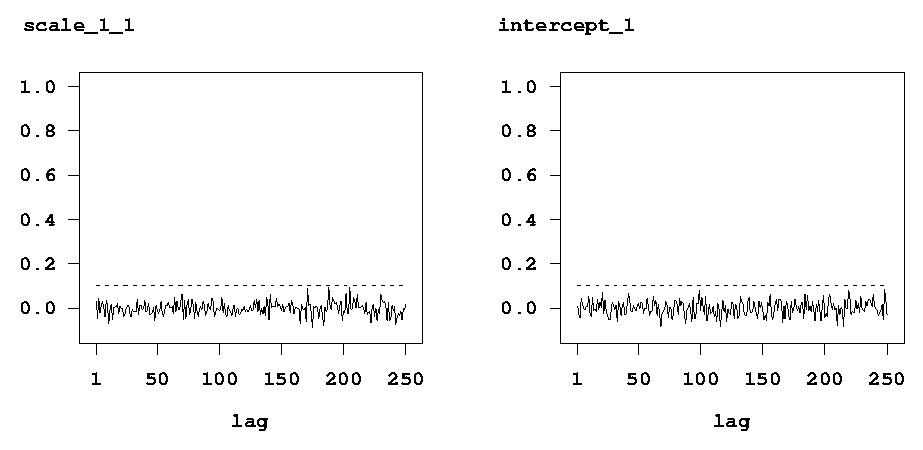
\epsfig{file=grafiken/zambia_mcmc_autocor1.eps,scale=0.75}
{\it\caption{Autocorrelation function for the scale parameter and
the intercept.\label{zambia_mcmc_autocor1}}}
\end{center}
\end{figure}

#> b.plotautocor, mean#

leads to the computation of only the minimum, mean and maximum
autocorrelation functions. The result for the scale parameter is
shown in \autoref{zambia_mcmc_autocor2}.

\begin{figure}[ht]
\begin{center}
\epsfig{file=grafiken/zambia_mcmc_autocormean1.ps,scale=0.5}
{\it\caption{Minimum, mean and maximum autocorrelation function
for the scale parameter.\label{zambia_mcmc_autocor2}}}
\end{center}
\end{figure}

Note, that executing the #plotautocor# command also stores the
computed autocorrelation functions in a file named #autocor.raw#
in the output directory of the {\it bayesreg object}.

To save memory, the sampling paths of the estimated parameters are
only stored temporarily by default and will be destroyed, when the
corresponding {\em bayesreg object} is deleted. If we want to
store the sampling paths permanently, we have to execute the
#getsample# command

#> b.getsample#

which stores the sampled parameters in ASCII files in the output
directory. To avoid too large files, the samples are typically
partitioned into several files. Executing the #getsample# command
also produces postscript files of the sampling paths in the output
directory (compare \autoref{zambia_mcmc_sample1} for the content
of one of these files).

\begin{figure}[ht]
\begin{center}
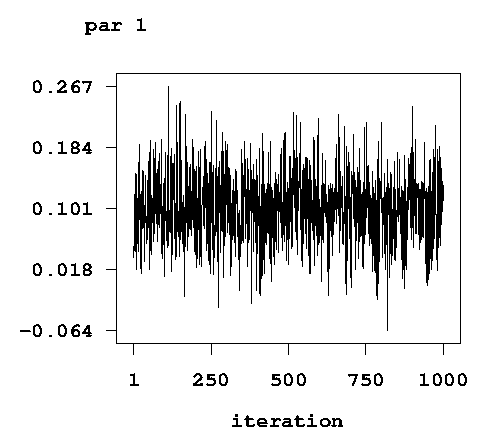
\epsfig{file=grafiken/zambia_mcmc_intercept_sample.eps,scale=0.75}
{\it\caption{Sampling path of the
intercept.\label{zambia_mcmc_sample1}}}
\end{center}
\end{figure}

\subsubsection{Sensitivity analysis}\label{zambia_mcmc_sensitivity}

In some situations the estimation results of a full Bayesian
semiparametric regression model depend on the choice of
hyperparameters, e.g.~the parameters #a# and #b# defining the
inverse gamma prior of the variances of nonparametric and spatial
effects. It is often recommended to check how sensitive the
results are with respect to changes in the hyperparameters. In the
following we will re-estimate the model from
\autoref{zambia_mcmc_regression} with different choices for the
hyperparameters #a# and #b# for each effect in the model. The
standard choices for #a# and #b# are #a=b=0.001#. As a first trial
we choose a smaller value for #a# and #b#:

#> b.regress hazstd = rcw + edu1 + edu2 + tpr + sex#\\
#  + bmi(psplinerw2,a=0.00001,b=0.00001) + agc(psplinerw2,a=0.00001,b=0.00001)#\\
#  + district(spatial,map=m,a=0.00001,b=0.00001)#\\
#  + district(random,a=0.00001,b=0.00001), family=gaussian iterations=12000#\\
#  burnin=2000 step=10 predict using d#


\autoref{zambia_mcmc_sensi1} shows the results for the
nonparametric effects with this choice of hyperparameters.
Obviously, the estimated functions are somewhat smoother but they
do not differ that much from the estimates with the standard
choices.

\begin{figure}[ht]
\begin{center}
\epsfig{file=grafiken/zambia_mcmc_f_bmi7.ps,scale=0.5}
\epsfig{file=grafiken/zambia_mcmc_f_age3.ps,scale=0.5} {\it\caption{Results
for the nonparametric effects with hyperparameters {\em\tt a=b=0.00001}
for nonparametric and spatial effects.\label{zambia_mcmc_sensi1}}}
\end{center}
\end{figure}

Now we try two further choices for the hyperparameters, with both
#a=1# and #b# small. We estimate models with #b=0.005# and
#b=0.00005#:

#> b.regress hazstd = rcw + edu1 + edu2 + tpr + sex + bmi(psplinerw2,a=1,b=0.005)#\\
#  + agc(psplinerw2,a=1,b=0.005) + district(spatial,map=m,a=1,b=0.005)#\\
#  + district(random,a=1,b=0.005), family=gaussian iterations=12000 burnin=2000#\\
#  step=10 predict using d#

#> b.regress hazstd = rcw + edu1 + edu2 + tpr + sex + bmi(psplinerw2,a=1,b=0.00005)#\\
#  + agc(psplinerw2,a=1,b=0.00005) + district(spatial,map=m,a=1,b=0.00005)#\\
#  + district(random,a=1,b=0.00005), family=gaussian iterations=12000 burnin=2000#\\
#  step=10 predict using d#

\autoref{zambia_mcmc_sensi2} and \autoref{zambia_mcmc_sensi3}
contain the results for the nonparametric effects for the two
choices of hyperparameters.

\begin{figure}[ht]
\begin{center}
\epsfig{file=grafiken/zambia_mcmc_f_bmi8.ps,scale=0.5}
\epsfig{file=grafiken/zambia_mcmc_f_age4.ps,scale=0.5} {\it\caption{Results
for the nonparametric effects with hyper parameters {\em\tt a=1} and
{\em\tt b=0.005} for nonparametric and spatial
effects.\label{zambia_mcmc_sensi2}}}
\end{center}
\end{figure}

\begin{figure}[ht]
\begin{center}
\epsfig{file=grafiken/zambia_mcmc_f_bmi9.ps,scale=0.5}
\epsfig{file=grafiken/zambia_mcmc_f_age5.ps,scale=0.5} {\it\caption{Results
for the nonparametric effects with hyper parameters {\em\tt a=1} and
{\em\tt b=0.00005} for nonparametric and spatial
effects.\label{zambia_mcmc_sensi3}}}
\end{center}
\end{figure}

\section{References}
\label{zambia_bayesregref}

\begin{description}

\item[Besag, J., Green, P., Higdon, D. and Mengersen, K. (1995):]
 Bayesian computation and stochastic systems (with discussion).
{\em Statistical Science}, 10, 3-66.

\item[Besag, J. and Kooperberg, C. (1995):] On conditional and intrinsic autoregressions.
{\em Biometrika}, 82, 733-746.

\item[Besag, J., York, J. and Mollie, A. (1991):]
Bayesian image restoration with two applications in spatial
statistics (with discussion). {\em Annals of the Institute of
Statistical Mathematics}, 43, 1-59.

\item[Biller, C. (2000):] {\em Bayesianische Ans\"atze zur nonparametrischen Regression.}
Skaker Verlag, Aachen.

\item[Brezger, A. (2000):] \href{http://www.stat.uni-muenchen.de/~andib}
{\em Bayesianische P-splines.} Master thesis, University of Munich.

\item[Brezger, A. and Lang, S. (2003):]
Generalized additive regression based on Bayesian P-splines. SFB
386 Discussion paper 321, Department of Statistics, University of
Munich. Conditionally accepted for {\em Computational Statistics and Data Analysis.}

\item[Clayton, D. (1996):] Generalized linear mixed models. In: Gilks, W., Richardson S. and
Spiegelhalter D. (eds), {\em Markov Chain Monte Carlo in
Practice}. London: Chapman and Hall, 275-301.

\item[Chen, M.H. and Dey, D.K. (2000):] Bayesian Analysis for Correlated Ordinal Data Models.
{\em Generalized linear models: A Bayesian perspective} (ed. Dey,
D.K., Ghosh, S.K. and Mallick, B.K.), 8,133-159, Marcel Dekker,
New York.

\item[Chib, S. and Greenberg, E. (1995):] Understanding the
Metropolis-Hastings Algorithm. {\em The American Statistician},
49, 327-335.

\item [Eilers, P.H.C.~and Marx, B.D. (1996):]
Flexible smoothing using B-splines and penalized likelihood (with
comments and rejoinder). {\it Statistical Science}, 11 (2),
89-121.

\item[Fahrmeir, L. and Lang, S. (2001a):]
Bayesian Inference for Generalized Additive Mixed Models Based on
Markov Random Field Priors. {\em Journal of the Royal Statistical
Society C}, 50, 201-220.

\item[Fahrmeir, L. and Lang, S. (2001b):] Bayesian Semiparametric Regression Analysis of Multicategorical
Time-Space Data. {\em Annals of the Institute of Statistical
Mathematics}, 53, 10-30.

\item[Fahrmeir, L. and Tutz, G. (2001):] {\em Multivariate Statistical
Modelling based on Generalized Linear Models.} New York:
Springer-Verlag.


\item[Gamerman, D. (1997):] Efficient Sampling from the posterior distribution
in generalized linear models. {\em Statistics and Computing}, 7,
57-68.

\item[Gelfand, A.E., Sahu, S.K. and Carlin, B.P. (1996):] Efficient Parametrizations for
Generalized Linear Mixed Models. In: Bernardo, J.M., Berger, J.O.,
Dawid, A.P. and Smith, A.F.M. (eds.), {\em Bayesian Statistics,
5}. Oxford University Press, 165-180.

\item[George, A. and Liu, J.W. (1981).] {\em Computer Solution of Large
Sparse Positive Definite Systems.} Series in computational
mathematics, Prentice-Hall.

\item[Green, P.J. (2001):] A Primer in Markov Chain Monte Carlo. In: Barndorff-Nielsen, O.E.,
Cox, D.R. and Kl{\"u}ppelberg, C. (eds.), {\em Complex Stochastic
Systems}. Chapmann and Hall, London, 1-62.

\item[Green, P.J. and Silverman, B. (1994):] {\em Nonparametric Regression and Generalized Linear Models.} Chapman
and Hall, London.

\item[Hastie, T. and Tibshirani, R. (1990):] {\em Generalized additive models.} Chapman and
Hall, London.

\item[Hastie, T. and Tibshirani, R. (1993):] Varying-coefficient Models.
{\em Journal of the Royal Statistical Society B}, 55, 757-796.

\item[Hastie, T. and Tibshirani, R. (2000):] Bayesian Backfitting. {\em Statistical Science}, 15, 193-223.

\item[Hastie, T., Tisbshirani, R. and Friedman, J. (2001):] {\em The Elements of Statistical Learning: Data Mining,
Inference and Prediction.} New York: Sprigner-Verlag.

\item[Knorr-Held, L. (1999):]
Conditional Prior Proposals in Dynamic Models. {\em Scandinavian
Journal of Statistics}, 26, 129-144.

\item[Kragler, P. (2000):] \href{http://www.scor.fr/us/2_laureat.asp?pays=2}
{Statistische Analyse von Schadensf\"allen privater
Krankenversicherungen.} Master thesis, University of Munich.


\item[Lang, S. (1996):]
\href{mailto:lang@stat.uni-muenchen.de} {Bayesianische Inferenz in
Modellen mit variierenden Koeffizienten}. Master thesis, University of Munich.


\item[Lang, S. and Brezger, A. (2004):]
Bayesian P-splines. {\em Journal of Computational and Graphical Statistics}, 13, 183-212.

\item[McCullagh, P. and Nelder, J.A. (1989):] {\em Generalized Linear Models.} Chapman and Hall, London.

\item[Rue, H. (2001):] Fast Sampling of Gaussian Markov Random Fields with Applications.
{\em Journal of the Royal Statistical Society B}, 63, 325-338.

\item[Spiegelhalter, D.J., Best, N.G., Carlin, B.P. and van der Linde, A. (2002):]
Bayesian measures of model complexity and fit. {\em Journal of the
Royal Statistical Society B}, 65, 583-639.

\end{description}
